\documentclass[11pt]{article}
\usepackage[T1]{fontenc}
\usepackage{lmodern}
\usepackage{microtype}
\usepackage[a4paper,margin=29mm]{geometry}
\usepackage{amsmath,amssymb,amsthm,mathtools}
\usepackage{enumitem}
\usepackage{booktabs}
\usepackage{tikz}
\usetikzlibrary{positioning,arrows.meta,calc}
\usepackage[numbers,sort&compress]{natbib}
\usepackage{xurl}
\usepackage[colorlinks=true,linkcolor=blue!45!black,citecolor=blue!45!black,
  urlcolor=blue!45!black,pdfauthor={OpenAI},
  pdftitle={The free energy of the Ising random perceptron}]{hyperref}
\usepackage{bookmark}
\numberwithin{equation}{section}
\newtheorem{theorem}{Theorem}[section]
\newtheorem{lemma}[theorem]{Lemma}
\newtheorem{proposition}[theorem]{Proposition}
\newtheorem{corollary}[theorem]{Corollary}
\theoremstyle{definition}
\newtheorem{definition}[theorem]{Definition}
\theoremstyle{remark}
\newtheorem{remark}[theorem]{Remark}
\setlist[enumerate]{itemsep=3pt,topsep=5pt}
\setlist[itemize]{itemsep=3pt,topsep=5pt}
\setcounter{tocdepth}{1}
\allowdisplaybreaks[1]
\emergencystretch=1em

\title{The free energy of the Ising random perceptron}
\author{OpenAI}
\date{September 24, 2026}
\begin{document}
\maketitle
\begin{abstract}
We determine the limiting free energy of the Ising perceptron with independent
Gaussian patterns for every bounded Borel log-potential, at every fixed positive
temperature and pattern density. We give an explicit variational formula for
the limit and prove convergence in expectation and probability.
\end{abstract}
\tableofcontents
\section{Introduction}\label{sec:introduction}

An Ising perceptron assigns a weight to each configuration
$x\in\{-1,1\}^N$ through its projections onto independent random patterns.
For Gaussian patterns $g^a\in\mathbb R^N$, a single projection is
$g^a\cdot x/\sqrt N$. Given a real log-potential $f$, the configuration
weight is the product of the factors $\exp f(g^a\cdot x/\sqrt N)$.
The logarithm of their uniform average, divided by $N$, measures the exponential scale
of the weighted configuration space. We use the uniform probability prior
on the cube and call this normalized log partition function the pressure.
The number of patterns is proportional to $N$, with fixed density
$\alpha>0$. Section~\ref{sec:model} gives the exact normalization.

This model combines a discrete configuration space with nonlinear random
constraints. At small density or weak interaction, a single typical overlap
can describe the pressure. More generally, a formula must retain the
distribution of overlaps between two samples from the Gibbs measure. The
patterns are Gaussian, but a nonlinear sum of their log-potentials is
generally not a Gaussian process indexed by the spins. Thus the Parisi
formula for Gaussian mixed $p$-spin Hamiltonians does not directly evaluate
this pressure.

\subsection{Storage models and rigorous predecessors}

The statistical-physics study of random-pattern storage was developed by
Gardner~\cite{gardner1988} and Gardner and Derrida~\cite{gardnerderrida1988}.
The latter work explicitly considered Ising couplings alongside spherical
ones. Krauth and M\'ezard~\cite{krauthmezard1989} analyzed the binary-coupling
model and predicted its storage capacity. In a storage problem a pattern
factor may be an indicator that a constraint is satisfied. At positive
temperature, a finite log-potential instead assigns a positive weight to
every configuration, allowing the pressure to measure both the pattern
reward and the number of configurations achieving it.

Talagrand established replica-symmetric formulas in small-density
perceptron regimes~\cite{talagrand2000halfspaces}. For Gaussian Ising
perceptrons with bounded Borel log-potentials, his high-temperature work
proved overlap-fluctuation bounds at sufficiently small
$\alpha$~\cite{talagrand2002}. Bolthausen, Nakajima, Sun, and
Xu~\cite{bolthausen2022gardner} later gave a new small-density proof of the
Gardner formula using first and second moments conditional on approximate
message passing. In their convention the activation is the multiplicative
weight $U=e^f$, up to constant rescaling. Their Theorem~1.1 treats measurable
weights satisfying a Gaussian-reweighted variance bound and
$\mathbb E[G U(G)]\ne0$; Remark~1.2 discusses the complementary zero-moment
case, where a direct second-moment argument applies. Their small-density
conclusions cover weights bounded above and away from zero, in particular
those arising from bounded real $f$. The density restrictions in these predecessors are
substantive and are absent from Theorem~\ref{thm:main}.

Hard constraints have a distinct, extensive theory. Ding and
Sun~\cite{dingsun2025} and Huang~\cite{huang2024capacity} proved matching
lower and upper capacity bounds at zero margin under their respective
explicit analytical conditions. Shmalo~\cite{shmalo2026capacity} subsequently
reported a computer-assisted verification of both conditions, yielding the
predicted zero-margin threshold; that preprint explicitly describes the
verification as a new proof claim not yet independently reproduced or peer
reviewed. Nakajima and Sun~\cite{nakajimasun2022}
proved concentration, sharp threshold sequences, and disorder universality
for broad hard-constraint classes. For symmetric interval constraints,
Perkins and Xu~\cite{perkinsxu2024} obtained entropy concentration and
freezing under an analytical condition; Abbe, Li, and
Sly~\cite{abbeli2021} proved a lognormal partition-function limit and removed
that condition, working with random-sign patterns. These results concern
specific zero-one weights. Such weights correspond to a log-potential
that takes the value $-\infty$, whereas the theorems here concern finite
log-potentials. A hard-constraint limit would require additional control
of the order of limits.

\subsection{The formula and its proof mechanisms}

Theorem~\ref{thm:main} evaluates the limiting Gaussian Ising pressure for
every fixed positive density and every bounded Borel real log-potential.
Writing $f=\beta\phi$ includes every fixed positive inverse temperature
$\beta$ for a bounded activation $\phi$. The variational parameter is a
nondecreasing overlap quantile $q:(0,1)\to[0,1]$. Its pattern contribution
is a Gaussian recursion, and its entropy contribution is the dual of the
one-spin $\log\cosh$ recursion. Section~\ref{sec:model} defines these
functionals before stating the theorem. No symmetry, concavity, or
smallness condition is imposed on the activation.

The proof uses the Ghirlanda--Guerra overlap
identities~\cite{gg1998}, Panchenko's ultrametricity
mechanism~\cite{panchenko2013}, and Ruelle probability
cascades~\cite{ruelle1987}. For Gaussian mixed-spin Hamiltonians,
Guerra's interpolation bound~\cite{guerra2003} led to Talagrand's proof
of the Parisi formula for even interactions~\cite{talagrand2006parisi};
Panchenko~\cite{panchenko2014parisi} subsequently included odd interactions
using ultrametricity.
We supply the array, duplication, and finite-cascade arguments needed
here. In particular, the changes of measure for the Gaussian marks are
proved with the conditioning required later. The joint transformation of
marks and cascade weights was developed by Panchenko and
Talagrand~\cite{panchenkotalagrand2007property,panchenkotalagrand2007interpolation}.

The hierarchical Gaussian-field enrichment is the construction used by
Mourrat and Panchenko~\cite{mourratpanchenko2020} to extend the Parisi
formula along a Hamilton--Jacobi equation. Our upper bound implements
Mourrat's contact-point supersolution strategy for nonconvex
interactions~\cite[Section~4]{mourrat2021}; see also its vector-spin
extension~\cite{mourrat2023upper}. In that strategy, a quadratic penalty
in perturbation parameters gives concentration and overlap identities
at deterministic contact points. Here the interaction parameter is the
Poissonized pattern density, whose derivative adds one nonlinear pattern.
Joint spin and cascade overlap identities, together with the
monotone-coupling argument of
synchronization~\cite{panchenko2015multispecies}, turn the field variations
at a contact point into the tail inequalities needed for this derivative.

The lower bound follows the cavity variational tradition of Aizenman,
Sims, and Starr~\cite{aizenmansimsstarr2003}. Its identification of the
cavity overlap as a derivative of the one-spin recursion is related to
the critical-point description developed by Chen and
Mourrat~\cite{chenmourrat2025}, and to the critical-point bounds of Chen,
Issa, and Mourrat~\cite[Section~6]{chenissamourrat2026}. Those results
concern Gaussian spin-glass Hamiltonians and do not directly evaluate the
nonlinear pattern model. In the present setting the Gaussian cavity
covariance must itself be identified from the bulk model. Two restored
patterns provide both first and second moments for that identification.

The companion article \emph{The free energy of the spherical random
perceptron}~\cite{spherical} develops the corresponding scalar enrichment
and two-pattern cavity strategy for spherical spins. Here all necessary
arguments are included, and the Ising prior requires its own entropy
calculation and cavity identity. The required concavity of the field
functional is the centered-Ising path-convexity theorem proved by Chen,
Issa, and Mourrat~\cite[Proposition~2.2]{chenissamourrat2026} and, by a
Parisi PDE argument, by Ho~\cite[Theorem~1.8]{ho2026concavity}, with the
opposite sign and a change of covariance normalization. We include a proof
covering repeated field levels and zero initial variance. Coordinate
exchangeability then identifies the cavity-spin overlap with the bulk
overlap. In the cascade calculation this identifies the dual subgradient;
the cited concavity turns this identity into attainment of the entropy
supremum. The model-specific task is to establish these identities for
the nonlinear perceptron.

\subsection{Organization of the proof}

The proof first treats smooth compactly supported log-potentials.
The two bounds use the variational paths differently. The upper comparison
starts from an arbitrary trial overlap path. The lower bound must instead
use the overlap path and field generated by the bulk model, and prove that
this field attains the entropy dual at that same overlap path.
Section~\ref{var:section} proves first variations, the tail order of the
pattern functional, and the field supporting inequality.
Section~\ref{arr:section} supplies the overlap-array and cascade laws.
The remaining stages are as follows.
\begin{enumerate}
 \item \emph{Upper comparison (Section~\ref{upper:section}).}
 Enrich the spins by cascade labels and hierarchical Gaussian fields,
 and Poissonize the number of patterns. If a proposed upper bound fails,
 an affine comparison has a negative minimum in a compact parameter
 region. A quadratic perturbation penalty gives fluctuation control at
 that deterministic minimum, yielding joint Ghirlanda--Guerra identities.
 These order the spin and label overlaps together. Field variations give
 tail inequalities that contradict the density derivative at the minimum.
 \item \emph{Restored covariances (Section~\ref{bulk:section}).}
 Enforce the overlap identities with two patterns omitted, then restore
 them as independent Gaussian marks. The marked-cascade calculation
 evaluates first and second moments of the empirical gradient covariance.
 It becomes a deterministic nondecreasing function of the limiting spin
 overlap; its diagonal and the dilation correction become deterministic
 as well.
 \item \emph{Cavity increments (Section~\ref{cav:section}).}
 Add a fixed number of Ising coordinates. A Taylor expansion and a
 normalized-measure estimate reduce the increment to a Gaussian cavity
 field and finitely many new patterns. Coordinate exchangeability
 identifies the entropy subgradient. Each limiting increment is bounded
 below by the variational value, up to the floor error in the pattern
 count. Averaging the perturbation parameters and telescoping then
 finishes the lower bound.
\end{enumerate}
The array calculations retain independent residual Gaussian noise on every
replica visit, including two visits to the same cascade leaf. This is needed
when the patterns are restored and when cavity-spin magnetizations are
evaluated; Figure~\ref{arr:residual-figure} illustrates the construction.

Finally, Section~\ref{sec:extensions} removes smoothness. Deleting one
pattern gives a Gaussian-$L^1$ approximation bound uniform in dimension;
the tilted recursion gives a matching bound uniform in the overlap path.
These estimates yield the bounded Borel theorem and the separately stated
integrable Gaussian extension. Entrywise replacement proves random-sign
universality under the stated Gaussian-null discontinuity condition.

\section{The model and the variational formula}\label{sec:model}

Fix a pattern density $\alpha>0$. Let $\nu_N$ be the uniform \emph{probability}
measure on $\{-1,1\}^N$, let $M_N=\lfloor\alpha N\rfloor$, and let
$g^1,\ldots,g^{M_N}$ be independent standard Gaussian vectors in
$\mathbb R^N$. For a bounded Borel function $f:\mathbb R\to\mathbb R$, put
\begin{equation}\label{def:pressure}
 b_a(x)=\frac{g^a\cdot x}{\sqrt N},\qquad
 Z_N(f)=\int\exp\!\left\{\sum_{a=1}^{M_N}f(b_a(x))\right\}\nu_N(dx),
 \qquad p_N(f)=\frac1N\log Z_N(f).
\end{equation}
The usual inverse temperature and activation are recovered by writing
$f=\beta\phi$, with $\beta>0$. Counting measure instead of $\nu_N$ adds
$\log2$ to the pressure. With either convention, physical free energy per
spin is the corresponding pressure multiplied by $-1/\beta$.

\subsection{Two finite Gaussian recursions}

An overlap path is a nondecreasing function $q:(0,1)\to[0,1]$. A trial field
path is a nonnegative nondecreasing step function $h:(0,1)\to[0,\infty)$
with finite values. Paths are identified up to equality almost everywhere;
all path integrals and $L^1$ norms use Lebesgue measure. Write $\mathcal Q$
for the overlap paths and $\mathcal H_{\mathrm{step}}$ for the trial fields.

A step path is described on a partition
\begin{equation}\label{def:partition}
 0=\zeta_0<\zeta_1<\cdots<\zeta_k=1,
 \qquad w_i=\zeta_{i+1}-\zeta_i,\quad 0\le i<k.
\end{equation}
Its value on $(\zeta_i,\zeta_{i+1})$ carries subscript $i$; repeated path
values are allowed. For a standard normal random variable $G$, define
\begin{equation}\label{def:transform}
 (\mathcal T_{s,d}U)(x)=
 \begin{cases}
 d^{-1}\log\mathbb E\exp\{dU(x+\sqrt s\,G)\},&d>0,\\
 \mathbb E U(x+\sqrt s\,G),&d=0,
 \end{cases}
 \qquad s\ge0,\quad 0\le d\le1.
\end{equation}

\begin{definition}[Pattern and field recursions]\label{def:recursions}
For a step overlap path $q$, append $q_{-1}=0$ and $q_k=1$. Starting at
$U_k=f$, set
\begin{equation}\label{def:pattern-recursion}
 U_{i-1}=\mathcal T_{q_i-q_{i-1},\zeta_i}U_i
 \quad(i=k,k-1,\ldots,0),\qquad V_f(q)=U_{-1}(0).
\end{equation}
For a step field path $h$, append $h_{-1}=0$. Starting instead at
$U_{k-1}(x)=\log\cosh x-h_{k-1}/2$, set
\begin{equation}\label{def:field-recursion}
 U_{i-1}=\mathcal T_{h_i-h_{i-1},\zeta_i}U_i
 \quad(i=k-1,k-2,\ldots,0),\qquad \ell(h)=U_{-1}(0).
\end{equation}
The letter $U$ refers to the recursion under discussion.
\end{definition}

The initial Gaussian average has coefficient $\zeta_0=0$. The pattern
recursion also has a final Gaussian average with coefficient $\zeta_k=1$
and variance $1-q_{k-1}$; the field recursion has no such extra interval.
For example, for constant paths $q(u)=r$ and $h(u)=H$,
\begin{align}
 V_f(r)&=\mathbb E_G\log\mathbb E_{G'}
   \exp f(\sqrt r\,G+\sqrt{1-r}\,G'),\label{def:one-level-pattern}\\
 \ell(H)&=\mathbb E\log\cosh(\sqrt H\,G)-H/2,
 \label{def:one-level-field}
\end{align}
where $G,G'$ are independent standard normals.

Subdividing an interval without changing its path value inserts a
zero-variance transform, so the definitions do not depend on the chosen
partition. For $f\in C_c^\infty(\mathbb R)$, the pattern functional is Lipschitz in the
$L^1$ distance between step paths. For bounded Borel $f$, it has a unique
continuous extension to $\mathcal Q$, constructed by uniform approximation
of the pattern functionals in Lemma~\ref{ext:path-approx}. We use that extension throughout. The field
functional is $1/2$-Lipschitz on step fields and therefore extends to bounded
nonnegative nondecreasing fields; see Proposition~\ref{var:continuity-order}.

\begin{definition}[Ising entropy]\label{def:entropy}
For $q\in\mathcal Q$, define the extended-valued functional
\begin{equation}\label{def:entropy-formula}
 S_{\mathrm I}(q)=\sup_{h\in\mathcal H_{\mathrm{step}}}
 \left\{\ell(h)+\frac12\int_0^1h(u)q(u)\,du\right\}.
\end{equation}
The field partition is independent of the overlap partition. In calculations
with two step paths, we always pass to a common refinement.
\end{definition}

\begin{theorem}[Gaussian Ising perceptron]\label{thm:main}
For every $\alpha>0$ and every bounded Borel $f:\mathbb R\to\mathbb R$,
\begin{equation}\label{thm:formula}
 \lim_{N\to\infty}\mathbb E p_N(f)
 =\mathcal P_f(\alpha)
 :=\inf_{q\in\mathcal Q}\{\alpha V_f(q)+S_{\mathrm I}(q)\}.
\end{equation}
Moreover, $p_N(f)$ converges to $\mathcal P_f(\alpha)$ in probability.
The variational value is finite. In particular, the conclusion holds for
$f=\beta\phi$ at every $\beta>0$ and every bounded continuous activation
$\phi$, without symmetry, concavity, or a smallness restriction.
\end{theorem}

The elementary bounds $S_{\mathrm I}\ge0$, $S_{\mathrm I}(0)=0$ and
$|V_f|\le\|f\|_\infty$ will be proved below. Since
$V_f(0)=\log\mathbb E e^{f(G)}$, they give
\begin{equation}\label{def:finite-value}
 -\alpha\|f\|_\infty\le\mathcal P_f(\alpha)
 \le\alpha\log\mathbb E e^{f(G)}.
\end{equation}
The proof of Theorem~\ref{thm:main} first assumes $f\in C_c^\infty(\mathbb R)$.
The upper bound is Proposition~\ref{upper:bound}, and
Proposition~\ref{cav:lower-bound} gives the matching lower bound.
Section~\ref{sec:extensions} removes smoothness
and proves the remaining convergence claims. It also gives extensions to
integrable unbounded activations and to independent random-sign patterns.

\subsection{Probabilistic conventions}

A Gibbs measure is a reference probability reweighted by an exponential
energy and then normalized. Replicas are independent samples from that
measure conditional on its disorder and reference data. Brackets
$\langle\cdot\rangle$ denote replica expectation, and $\mathbb E$ averages
the disorder and any explicitly introduced random data. A deterministic
perturbation parameter is held fixed under $\mathbb E$ unless its averaging
is specified. The spin overlap is
\[
 R(x,x')=N^{-1}x\cdot x',\qquad R_{ab}=R(x^a,x^b).
\]
An array limit means convergence in law of every finite sampled restriction,
including disorder averaging. All constants may depend on $\alpha$ and the
fixed smooth activation. Dependence on a fixed number of cavity coordinates
$L$ is allowed only where indicated; the limit in $N$ is always taken before
letting $L$ increase.

\section{Variations, order, and the Ising entropy}
\label{var:section}

Let $f\in C_c^\infty(\mathbb R)$. The upper bound will use two
properties of the variational formula: increasing the tail integrals of
an overlap path decreases $V_f$, and finite step trials with top value
below one suffice for the infimum. The lower bound needs a different
property: concavity of $\ell$ turns its first variation into a global
supporting inequality, which will identify the entropy supremum.
We establish these properties from the recursions of
Definition~\ref{def:recursions}.

Recall their different endpoints:
the pattern recursion has $q_{-1}=0$, $q_k=1$, and coefficients
$\zeta_0=0,\ldots,\zeta_k=1$, whereas the field recursion has
terminal value $\log\cosh(x)-h_{k-1}/2$ and stops at level $k-1$.
Inserting a partition point without changing a step value inserts an
identity transform of variance zero. Consequently either recursion may
be computed on any common refinement of the partitions in use.

\subsection{First variations and the pattern tail order}

For either recursion write $s_i$ for its variance increment and define
the probability kernel
\begin{equation}
\label{var:kernel}
 K_i(x,dy)=
 \exp\{\zeta_i(U_i(y)-U_{i-1}(x))\}
 \mathcal N(x,s_i)(dy).
\end{equation}
Here $s_i=q_i-q_{i-1}$, $0\le i\le k$, in the pattern
recursion, and $s_i=h_i-h_{i-1}$, $0\le i\le k-1$, in
the field recursion. The normalization follows directly from the
definition of $\mathcal T_{s_i,\zeta_i}$; when $\zeta_i=0$
the exponential is one. A zero-variance kernel is the point mass at
its starting point. Let $Z_{-1}=0$ and, successively, sample $Z_i$
from $K_i(Z_{i-1},\cdot)$.

Two elementary derivative identities will be used repeatedly. For a
smooth terminal function $U$, put $W=\mathcal T_{s,d}U$ and let
$K$ denote the corresponding tilted Gaussian kernel. Differentiation
in $x$ and in a perturbation $U+\varepsilon A$ gives
\begin{equation}
\label{var:transform-derivatives}
 W'=K U',\qquad
 \left.\frac{d}{d\varepsilon}
 \mathcal T_{s,d}(U+\varepsilon A)\right|_{\varepsilon=0}=K A.
\end{equation}
The Gaussian heat equation gives
\begin{equation}
\label{var:generator}
 \partial_s W
 =\frac12\{W''+d(W')^2\}
 =\frac12 K\{U''+d(U')^2\}.
\end{equation}
For $d>0$, these identities follow by differentiating
$e^{dW}=\mathbb E e^{dU(x+\sqrt sG)}$; for $d=0$ they
are the ordinary heat-semigroup identities. In particular,
$U_i'(Z_i)$ is a martingale along the tilted chain, since
$K_iU_i'=U_{i-1}'$.

\begin{lemma}[First variations]
\label{var:variation}
On a fixed partition with $w_i=\zeta_{i+1}-\zeta_i$, the first
variations along every feasible line segment of step paths are
\begin{align}
\label{var:pattern-variation}
 \frac{d}{da}V_f(q+a\dot q)
 &=-\frac12\sum_{i=0}^{k-1}w_i\dot q_i\,
   \mathbb E[U_i'(Z_i)^2],\\
\label{var:field-variation}
 \frac{d}{da}\ell(h+a\dot h)
 &=-\frac12\sum_{i=0}^{k-1}w_i\dot h_i\,
   \mathbb E[U_i'(Z_i)^2].
\end{align}
The functions and chains on the right are computed at the current
path. Endpoint derivatives are understood from within the segment.
The squared-derivative expectations on the right are continuous on the
closed finite-dimensional parameter cones. In both recursions these
expectations are nonnegative and nondecreasing in $i$. In the field
recursion, define
\begin{equation}
\label{var:rho}
 \rho_h(u)=\rho_i:=\mathbb E[U_i'(Z_i)^2],
 \qquad \zeta_i<u<\zeta_{i+1}.
\end{equation}
Then $0\le\rho_h\le1$, and subdivision does not change this path.
\end{lemma}

\begin{proof}
First suppose all variance increments being differentiated are
strictly positive. Moving $q_i$ lengthens the transition ending at
level $i$ and shortens the transition leaving that level. By
\eqref{var:generator}, the incoming derivative, expressed at level
$i$ before propagation through the preceding kernels, is
$\{U_i''+\zeta_i(U_i')^2\}/2$. The outgoing derivative is
$-\{U_i''+\zeta_{i+1}(U_i')^2\}/2$. Their sum is
$-w_i(U_i')^2/2$. Formula~\eqref{var:transform-derivatives}
propagates this sum through the kernels ending at levels
$i,i-1,\ldots,0$, giving
$\partial_{q_i}V_f=-w_i\mathbb E[U_i'(Z_i)^2]/2$.

The same cancellation applies to $h_i$ for $i<k-1$.
At the last field level the incoming derivative and the derivative
of the subtraction $-h_{k-1}/2$ combine to give
\[
 \frac12\{(\log\cosh)''+
            \zeta_{k-1}((\log\cosh)')^2-1\}
 =-\frac{1-\zeta_{k-1}}2\tanh^2.
\]
This is the same formula with $w_{k-1}=1-\zeta_{k-1}$.
Linearity yields both displayed variations.

For completeness, the differentiations remain valid at degenerate
increments. A Gaussian transform of either terminal function is
smooth in the spatial variable and has bounded derivatives of every
positive order. This follows inductively by differentiating the
tilted expectation: the resulting terms are finite sums of tilted
moments of products of bounded derivatives of the next-level
function. The functions themselves are bounded in the pattern
case and have at most linear growth in the field case. On every
compact variance-parameter set, the Gaussian exponential moments
therefore dominate all terms in these formulas. Coupling the
increments as $\sqrt{s_i}G_i$ shows continuity as any $s_i$
decreases to zero, both for recursion values and for the tilted
moments that appear above. The heat-equation identity also has
this continuous extension because its spatial derivatives do.
Approximate the endpoints of a feasible segment by interior points
on a common partition and integrate the already proved derivative
formula along the approximating segments. Dominated convergence
gives the same integral formula on the original segment and its
one-sided endpoint derivatives.

Finally, the derivative martingale and conditional Jensen inequality
show that its second moments increase with the level. The terminal
derivative bounds are $\|f'\|_\infty$ and $1$, respectively;
the same bounds hold at every earlier level by
\eqref{var:transform-derivatives}. An inserted zero-variance
transition repeats the same derivative and chain value, so it
does not change $\rho_h$.
\end{proof}

\begin{proposition}[Continuity and tail order]
\label{var:continuity-order}
For step paths on arbitrary partitions,
\begin{align}
\label{var:lipschitz}
 |V_f(p)-V_f(q)|&\le\tfrac12\|f'\|_\infty^2\|p-q\|_{L^1},\\
 |\ell(h')-\ell(h)|&\le\tfrac12\|h'-h\|_{L^1}.
\end{align}
Thus $V_f$ extends uniquely and continuously to all nondecreasing
$[0,1]$-valued paths, and $\ell$ extends to all bounded
nonnegative nondecreasing paths. Moreover,
\begin{equation}
\label{var:tail-order}
 \int_s^1p(u)\,du\ge\int_s^1q(u)\,du
 \quad\hbox{for every }s\in[0,1]
 \quad\Longrightarrow\quad V_f(p)\le V_f(q).
\end{equation}
\end{proposition}

\begin{proof}
Refine the two partitions and integrate
Lemma~\ref{var:variation} along the segment joining the paths.
The terminal derivative bounds give \eqref{var:lipschitz}.
Step paths are dense in the indicated classes in $L^1$, which
gives the extensions.

For the order assertion on a common partition, set
$a_i=w_i(p_i-q_i)$ and $A_j=\sum_{i=j}^{k-1}a_i$.
The hypothesis gives $A_j\ge0$. For every nonnegative
nondecreasing sequence $c_i$,
\begin{equation}
\label{var:summation-parts}
 \sum_{i=0}^{k-1}a_ic_i
 =c_0 A_0+\sum_{j=1}^{k-1}(c_j-c_{j-1})A_j\ge0.
\end{equation}
At each point of the segment from $q$ to $p$, take
$c_i=\mathbb E[U_i'(Z_i)^2]$ and apply
\eqref{var:pattern-variation}. The derivative along the segment
is nonpositive, proving the claim for steps.

For general paths, replace each by its average on each interval of
a common sequence of successively finer uniform partitions.
These averages are nondecreasing and converge in $L^1$ to the
original paths. Their tail-integral differences at partition
boundaries equal the original differences. Between boundaries
the differences are affine and hence nonnegative as well.
Apply the step result and then \eqref{var:lipschitz}.
\end{proof}

\begin{corollary}[Finite variational value and reduction to finite trials]
\label{var:step-reduction}
The entropy in Definition~\ref{def:entropy} is nonnegative,
nondecreasing in pointwise path order, and satisfies
$S_{\mathrm I}(0)=0$. The variational infimum is finite, and
\begin{equation}
\label{var:step-infimum}
 \inf_q\{\alpha V_f(q)+S_{\mathrm I}(q)\}
 =\inf_{\substack{q\text{ step}\\q_{k-1}<1}}
       \{\alpha V_f(q)+S_{\mathrm I}(q)\}.
\end{equation}
\end{corollary}

\begin{proof}
The trial $h=0$ gives $S_{\mathrm I}(q)\ge0$. Each expression
in its defining supremum is nondecreasing in $q$ because $h\ge0$.
Also $\ell(0)=0$ and \eqref{var:field-variation}, integrated
along $a\mapsto ah$, gives $\ell(h)\le0$, whence
$S_{\mathrm I}(0)=0$. Every transform preserves the range of a
bounded terminal function, so $|V_f(q)|\le\|f\|_\infty$.
In fact, the zero path has
$V_f(0)=\log\mathbb E e^{f(G)}$. These observations bound the
infimum below by $-\alpha\|f\|_\infty$ and provide a finite
upper bound using $q=0$.

For any quantile $q$, let $\underline q_m$ on each interval of
the uniform $m$-partition be $(1-1/m)$ times the essential
infimum of $q$ on that interval. Then
$0\le\underline q_m\le q$ almost everywhere,
$\sup\underline q_m<1$, and
$\|\underline q_m-q\|_{L^1}\to0$. The last assertion follows,
for example, from convergence at every continuity point of a
monotone representative, followed by bounded convergence.
Consequently $S_{\mathrm I}(\underline q_m)\le S_{\mathrm I}(q)$,
while $V_f(\underline q_m)\to V_f(q)$.
Taking a limit superior for each finite-entropy trial $q$ proves
the nontrivial inequality in \eqref{var:step-infimum}; the other
inequality follows from inclusion of the trial classes. No
continuity assertion for the extended-valued entropy is needed.
\end{proof}

\subsection{Concavity of the field recursion}

The supporting inequality below is the property of the centered Ising
spin law used in the lower bound. Its concavity statement is the
path-convexity theorem of Chen, Issa, and
Mourrat~\cite[Propositions~2.2 and~2.4]{chenissamourrat2026}: with their
notation and covariance normalization, $\ell(h)=-\psi_{\circ}(h/2)$.
Ho~\cite[Theorem~1.8]{ho2026concavity} proves the same path-convexity
statement through a concavity theorem for the time-changed Parisi PDE.
This is convexity along linear interpolations of quantile paths, not
along affine interpolations of their probability laws. The proof below
uses the Hessian criterion of Chen, Issa, and Mourrat: the negative Hessian has nonpositive
off-diagonal entries and nonnegative row sums. We derive the
off-diagonal signs directly from folded Gaussian kernels and include
the extension to repeated or zero field levels. The preservation of
even functions monotone in absolute value by these transitions is
classical; see Panchenko~\cite[Lemma~2(d)]{panchenko2005question}.
The next lemma gives a direct proof in the form needed here.

\begin{lemma}[Order preservation by a folded transition]
\label{var:folded-kernel}
Suppose $U:\mathbb R\to\mathbb R$ is even and convex. Let $K$ be
its tilted Gaussian kernel with variance $s\ge0$ and coefficient
$d\ge0$, and assume its normalizer
$\mathbb E e^{dU(x+\sqrt sG)}$ is finite for every $x\in\mathbb R$.
If $A$ is bounded, even, and nondecreasing in $|x|$, then $KA$
has these properties as well. The same statement with
``nonincreasing'' holds with both monotonicities reversed.
\end{lemma}

\begin{proof}
Evenness follows by reflection, and $s=0$ is immediate. For
$s>0$, the law of the next absolute value $y\ge0$ when the
starting point is $x\ge0$ has density proportional to
\[
 e^{-y^2/(2s)}\cosh(xy/s)e^{dU(y)}.
\]
For $x_2\ge x_1\ge0$, the ratio of these normalized densities
is a positive constant times
$\cosh(x_2y/s)/\cosh(x_1y/s)$. Its logarithmic derivative in
$y$ is
\[
 \frac{x_2}{s}\tanh(x_2y/s)
 -\frac{x_1}{s}\tanh(x_1y/s)\ge0,
\]
because $x\mapsto x\tanh(xy/s)$ is nondecreasing on
$[0,\infty)$. Thus the density ratio $L(y)$ is increasing.
If $Y,Y'$ are independent with the law corresponding to $x_1$,
then
\[
 \operatorname{Cov}(A(Y),L(Y))
 =\tfrac12\mathbb E[(A(Y)-A(Y'))(L(Y)-L(Y'))]\ge0.
\]
Since $\mathbb E L(Y)=1$, this proves
$K A(x_2)\ge K A(x_1)$. Negating $A$ proves the reversed
statement. The normalizations are included in $L$ and do not
alter its monotonicity.
\end{proof}

\begin{theorem}[Concavity and a supporting field]
\label{var:concavity}
The functional $\ell$ is concave on nonnegative nondecreasing
step paths. For any two such paths, represented on a common
partition,
\begin{equation}
\label{var:support}
 \ell(h')\le\ell(h)
      -\frac12\int_0^1(h'(u)-h(u))\rho_h(u)\,du.
\end{equation}
Concavity also holds for its continuous extension to bounded
nonnegative nondecreasing paths.
\end{theorem}

\begin{proof}
Fix a partition. We first work in its open cone
$0<h_0<h_1<\cdots<h_{k-1}$, where all parameter derivatives
below exist. Write $m_i=U_i'$ and
$\rho_i=\mathbb E m_i(Z_i)^2$ as in \eqref{var:rho}.
By the first variation, the matrix
\[
 A_{ij}=w_i\partial_{h_j}\rho_i
       =-2\partial_{h_j}\partial_{h_i}\ell
\]
is symmetric. We will prove that its off-diagonal entries are
nonpositive and its row sums are nonnegative. These two properties
make $A$ positive semidefinite, as the decomposition
\eqref{var:psd} below shows. They correspond to increasing one later
field level and to increasing all field levels together, respectively.

Every $U_i$ is even and convex. Evenness is preserved by the
Gaussian transforms. To check convexity when $d>0$, use convexity
of $U$ and H\"older's inequality to obtain, for $0\le a\le1$,
\[
 \mathbb E e^{dU(ax+(1-a)y+\sqrt sG)}
 \le
 (\mathbb E e^{dU(x+\sqrt sG)})^a
 (\mathbb E e^{dU(y+\sqrt sG)})^{1-a}.
\]
Taking logarithms proves convexity of the transform; expectation
preserves it when $d=0$. The terminal subtraction is constant in
$x$ and does not affect the argument. In particular, $m_i$ is
odd, $m_i(x)\ge0$ for $x\ge0$, and $m_i(x)^2$ is even and
nondecreasing in $|x|$. All $U_i$ have at most linear growth, so
the normalizers in Lemma~\ref{var:folded-kernel} are finite.

We first establish the cross-derivative sign
\begin{equation}
\label{var:cross-sign}
 \partial_{h_j}\rho_i\le0\qquad(j>i).
\end{equation}
Repeat the switch calculation from Lemma~\ref{var:variation},
but stop its backwards propagation at the function $U_i(x)$.
This gives
\begin{equation}
\label{var:later-switch}
 \partial_{h_j}U_i(x)
 =-\frac{w_j}{2}
   (K_{i+1}\cdots K_j m_j^2)(x),\qquad j>i.
\end{equation}
Lemma~\ref{var:folded-kernel} says that this function is even
and nonincreasing in $|x|$. Its derivative is therefore
nonpositive for $x>0$ and nonnegative for $x<0$. Since $m_i$
has the opposite signs, the direct derivative of the terminal
test in the expression $\rho_i=K_0\cdots K_i(m_i^2)(0)$ is
pointwise nonpositive:
\[
 \partial_{h_j}(m_i^2)
   =2m_i(\partial_{h_j}U_i)'\le0.
\]

It remains to account for all derivatives of the probability
kernels in this expression. If $l\le i<j$, the variance of
$K_l$ is independent of $h_j$. Put
$A_l=\partial_{h_j}U_l$. Differentiating the normalized kernel
at a fixed starting point gives the score
\begin{equation}
\label{var:kernel-score}
 \partial_{h_j}\log K_l(x,dy)
 =\zeta_l\{A_l(y)-(K_lA_l)(x)\}.
\end{equation}
Indeed the derivative of $U_{l-1}$ in its normalizing factor
equals $K_l A_l$, by
\eqref{var:transform-derivatives}. In the product rule for
$K_0\cdots K_i(m_i^2)$, the test at level $l$ is
$H_l=K_{l+1}\cdots K_i(m_i^2)$, with $H_i=m_i^2$.
It is even and nondecreasing in absolute value by
Lemma~\ref{var:folded-kernel}. On the other hand, $A_l$ is even
and nonincreasing in absolute value by
\eqref{var:later-switch}. Thus differentiating this kernel
contributes, at its starting point,
\[
 \zeta_l\operatorname{Cov}_{K_l(x,\cdot)}(H_l,A_l)\le0.
\]
The sign follows from the same independent-copy covariance
identity as in Lemma~\ref{var:folded-kernel}, now for two
functions of $|y|$ with opposite monotonicities. Propagation
through preceding probability kernels preserves the sign.
This includes $l=0$, whose score is zero because $\zeta_0=0$.
Together with the direct derivative, these are all terms in the
product rule, proving \eqref{var:cross-sign}.

Next increase every field value by the same number $a\ge0$.
All increments after level zero remain unchanged. Each $U_i$,
$i\ge0$, changes only by the additive constant $-a/2$, so its
spatial derivative and all kernels $K_l$ for $l\ge1$ remain
unchanged. The sole change in the chain is that its first,
untilted Gaussian variance increases from $h_0$ to $h_0+a$.
The function
$K_1\cdots K_i(m_i^2)$ is even and nondecreasing in absolute
value. Coupling the initial values as
$\sqrt{h_0+a}G$ therefore proves
\begin{equation}
\label{var:row-sum}
 \sum_{j=0}^{k-1}\partial_{h_j}\rho_i\ge0.
\end{equation}

We can now apply the matrix criterion. By \eqref{var:cross-sign}
and symmetry every off-diagonal entry of $A$ is nonpositive,
and \eqref{var:row-sum} gives nonnegative row sums. For every
$v\in\mathbb R^k$,
\begin{equation}
\label{var:psd}
 v^{\mathsf T}Av
 =\sum_i\left(\sum_jA_{ij}\right)v_i^2
   +\sum_{i<j}(-A_{ij})(v_i-v_j)^2\ge0.
\end{equation}
Thus the Hessian of $\ell$ is negative semidefinite on the
open cone. Restricting $\ell$ to a line segment in that cone
proves concavity and, using its derivative at the starting
point, the inequality \eqref{var:support} there.

For arbitrary field steps $h,h'$ on this partition, replace
$h_i,h_i'$ by $h_i+\varepsilon(i+1)$ and
$h_i'+\varepsilon(i+1)$. Both perturbed paths lie in the open
cone and their difference remains $h'-h$. Let
$\varepsilon\downarrow0$. The value and coefficient continuity
in Lemma~\ref{var:variation} proves both concavity and
\eqref{var:support} on the closed cone. Common refinement
handles distinct partitions. Finally, approximate any two
bounded field paths in $L^1$ by monotone steps on common
partitions and use Proposition~\ref{var:continuity-order} to
pass the concavity inequality to their limits.
\end{proof}

For a step field $h$, the supporting inequality gives the concrete
entropy identity
\[
 S_{\mathrm I}(\rho_h)
 =\ell(h)+\frac12\int_0^1h(u)\rho_h(u)\,du.
\]
Indeed, adding $\frac12\int h'\rho_h$ to \eqref{var:support}
bounds every trial value by the value at $h$, and $h$ itself is
admissible. The nonlinear model must still identify its overlap path
with this field derivative. Section~\ref{cav:section} obtains that
identity from coordinate exchangeability and passes the same supporting
inequality to the bounded field produced by the cavity limit.

\section{Overlap arrays and probability cascades}
\label{arr:section}

Fresh Gaussian patterns are determined on finitely many replicas by their
overlap covariance matrices.  This lets us evaluate their contribution
from limiting array laws, without representing an arbitrary limiting Gibbs
measure.  We first derive the ultrametric structure forced by the
Ghirlanda--Guerra identities and realize its finite approximations by
probability cascades.  We then compute how Gaussian marks change when a
cascade is reweighted.  Finally, Lemma~\ref{arr:limit} expresses the
reciprocal normalizers of bounded reweightings as limits of polynomials;
each polynomial uses only finitely many replicas.  Thus disorder-averaged
array laws suffice even for these normalized expectations.

All array laws in this section include the disorder average.  In particular,
the conditional overlap identities below condition on a sampled array
block, not on a fixed realization of the disorder.

For a Gibbs probability, replicas are independent samples conditional on its
reference data and disorder; their conditional expectation is denoted by
$\langle\cdot\rangle$.  The expectation $\mathbb E$ also averages the disorder
and any additional randomness specified in the construction.  A symmetric
array $B=(B_{\ell m})_{\ell,m\geq1}$ is \emph{weakly exchangeable} if its law is
invariant under every finite permutation of the indices, and is a
\emph{Gram array} if every finite restriction is positive semidefinite.
These properties, and a fixed diagonal, pass to limits in distribution of
finite restrictions.  Bounded arrays admit such subsequential limits.

\subsection{Conditional identities, positivity, and duplication}

The overlap-mixture identities originate in the work of Ghirlanda and
Guerra~\cite{gg1998}.  Their occurrence in the present models will be
proved by the Gaussian perturbations in the upper and lower bounds.

\begin{definition}[Ghirlanda--Guerra property]
\label{arr:gg}
Let $B$ be a weakly exchangeable array with values in a compact space, and
write $\mu=\mathcal L(B_{12})$.  We say that $B$ has the
Ghirlanda--Guerra property if, for every $n\geq2$,
\begin{equation}
 \mathcal L\bigl(B_{1,n+1}\mid (B_{\ell m})_{\ell,m\leq n}\bigr)
 =\frac1n\mu+\frac1n\sum_{\ell=2}^n\delta_{B_{1\ell}}.
 \label{arr:conditional-gg}
\end{equation}
Equivalently, for every bounded measurable function $F$ of the first
$n\times n$ block and every bounded measurable $\psi$,
\begin{equation}
 \mathbb E[F\psi(B_{1,n+1})]
 =\frac1n\mathbb E[F]\mathbb E[\psi(B_{12})]
  +\frac1n\sum_{\ell=2}^n\mathbb E[F\psi(B_{1\ell})].
 \label{arr:gg-tested}
\end{equation}
The same definition applies to a joint array, with $B_{\ell m}$ a tuple of
entries.  By exchangeability the distinguished index $1$ can be replaced
by any of the first $n$ indices.
\end{definition}

It suffices to establish \eqref{arr:gg-tested} for continuous $F,\psi$:
the equality then identifies the relevant finite measures, and hence holds
for bounded measurable tests.  This observation also proves that the
property passes to weak limits on a compact entry space.  A measurable
entrywise image of a joint array retains the property, with conditioning
on its own first block, by the conditional-expectation tower rule.

The direct array argument below uses duplication, the mechanism in
Panchenko's ultrametricity proof~\cite[Theorem~4 and Section~3]{panchenko2013}.

\begin{theorem}[Positivity and ultrametricity]
\label{arr:ultrametric}
Suppose $B$ is a bounded, symmetric, weakly exchangeable Gram array with
constant diagonal $D$ and the Ghirlanda--Guerra property.  Then, almost
surely, for distinct indices,
\begin{equation}
 B_{\ell m}\geq0,
 \qquad
 B_{12}\geq\min\{B_{13},B_{23}\}.
 \label{arr:ultrametric-inequality}
\end{equation}
\end{theorem}

\begin{proof}
First suppose $b=\mathbb P(B_{12}<-\varepsilon)>0$ for some
$\varepsilon>0$.  On the event that all distinct pairs among the first
$n$ indices have overlap below $-\varepsilon$, each of the $n$ links to
index $n+1$ fails this condition with conditional probability
$(1-b)/n$, by \eqref{arr:conditional-gg}.  A union bound therefore gives
conditional probability at least $b$ that all the new links satisfy it.
Starting with $n=2$, such blocks have positive probability for every size.
Their quadratic form on the all-ones vector is at most
$nD-n(n-1)\varepsilon$, contradicting positive semidefiniteness for large
$n$.  Taking a countable sequence of $\varepsilon$ proves positivity.

We next prove a support duplication assertion.  If
$(a_{\ell m})_{\ell,m\leq n}$ belongs to the support of a finite block,
$n\geq2$, there is a supported extension to $n+1$ such that
\begin{equation}
 a_{i,n+1}=a_{in}\quad(i<n),\qquad
 a_{n,n+1}\leq\max_{i<n}a_{in}.
 \label{arr:duplication}
\end{equation}
Fix $b_*>\max_{i<n}a_{in}$ and a positive-probability neighborhood event
$A$ for the first $n$ indices, chosen so that all specified links to $n$
are below $b_*$.  Let $A_0$ impose just the restrictions among the first
$n-1$ indices.  An index $j\geq n$ \emph{matches} if its links to those
$n-1$ indices belong to the neighborhoods prescribed for $n$.  Thus
$A=A_0\cap\{n\text{ matches}\}$.

Suppose that, on $A$, a fresh index cannot both match and have its link to
$n$ below $b_*$.  Let $W_B$ be the limiting empirical frequency of
matching indices, and $W$ the frequency of indices $j>n$ with
$B_{nj}\geq b_*$.  These frequencies exist in $L^2$.  Indeed, for an
exchangeable sequence of indicators the second moments of empirical
averages and their mixed second moments have the same limit, so the
averages are $L^2$-Cauchy.  The limits are unchanged by finite
permutations of the relevant unobserved indices.  The supposition and
exchangeability imply $W_B\leq W$ on $A$.

Put $b=\mathbb P(B_{12}\geq b_*)$.  We have $b<1$, since $A$ has positive
probability and specifies links below $b_*$.  Conditional on $A$, the
first high link to $n$ has probability $b/n$; after $j$ consecutive high
links the next has probability $(b+j)/(n+j)$.  Applying
\eqref{arr:conditional-gg} successively, and then expressing empirical
frequency moments by products at distinct fresh indices, gives
\begin{equation}
 \mathbb E[\mathbf1_A W^d]
 =\mathbb P(A)\prod_{j=0}^{d-1}\frac{b+j}{n+j},
 \qquad d\geq1.
 \label{arr:duplication-moments}
\end{equation}
The binomial series therefore yields
\begin{equation}
 \mathbb E[\mathbf1_A(1+zW)^{-n}]
 =\mathbb P(A)(1+z)^{-b},\qquad z>0.
 \label{arr:duplication-transform}
\end{equation}
Initially the series proves this for $0<z<1$.  Both sides are real
analytic on $(0,\infty)$, the left side by boundedness of $W$ and local
power-series domination, so the identity holds throughout that interval.
It also includes $b=0$.

To compare the matching frequency with the high-link frequency, write
$I_j=\mathbf1_{\{j\text{ matches}\}}$.  The event $A_0$ uses only the
first $n-1$ indices, and $W_B$ is unchanged by every finite permutation
of the remaining indices, including index $n$.  Hence, for every bounded
continuous $\varphi$, exchangeability gives
\[
 \mathbb E[\mathbf1_{A_0}I_n\varphi(W_B)]
 =\mathbb E\left[\mathbf1_{A_0}
   \frac1M\sum_{j=n}^{n+M-1}I_j\varphi(W_B)\right]
 \longrightarrow
 \mathbb E[\mathbf1_{A_0}W_B\varphi(W_B)].
\]
The limit uses the $L^2$ convergence defining $W_B$; adding index $n$
does not change that frequency.  Taking
$\varphi(x)=(1+zx)^{-n}$ and using $W_B\le W$ on $A$ now gives
\begin{align}
 \mathbb E[\mathbf1_A(1+zW)^{-n}]
 &\leq\mathbb E[\mathbf1_A(1+zW_B)^{-n}]\notag\\
 &=\mathbb E[\mathbf1_{A_0}W_B(1+zW_B)^{-n}]
 \leq z^{-1}.
 \label{arr:duplication-contradiction}
\end{align}
The last bound uses $x/(1+zx)^n\leq1/z$.  Equations
\eqref{arr:duplication-transform} and
\eqref{arr:duplication-contradiction} contradict $b<1$ as $z\to\infty$.
Consequently the desired extension event has positive probability.
Shrinking the neighborhoods and decreasing $b_*$ to its target value,
compactness of the bounded finite-block support proves
\eqref{arr:duplication}.  Permutation symmetry permits duplication of
any chosen index.

If ultrametricity failed, a supported triple could be chosen with
$a_{12}<a_{13}\leq a_{23}$.  Repeated duplication makes three groups of
$m$ indices, preserving the three cross-group entries $a_{12},a_{13},a_{23}$.
Within each group all off-diagonal entries stay at most its largest
cross-group entry: this follows inductively from
\eqref{arr:duplication}.  Represent the resulting finite Gram matrix by
vectors and let $u_1,u_2,u_3$ be their group averages.  Then
\[
 \|u_2\|^2,\|u_3\|^2
 \leq \frac Dm+\left(1-\frac1m\right)a_{23},
 \qquad u_2\cdot u_3=a_{23},\qquad \|u_1\|\leq\sqrt D.
\]
Hence $\|u_2-u_3\|^2\leq2(D-a_{23})/m\to0$, whereas
$u_1\cdot(u_3-u_2)=a_{13}-a_{12}>0$.  Cauchy--Schwarz gives a
contradiction.  Applying exchangeability to all triples completes the
proof.
\end{proof}

\subsection{Finite cascades and their sampling law}

The hierarchical weights defined next are finite Ruelle probability
cascades~\cite{ruelle1987}. Their complete weights-and-ancestry sampling
law was identified by Bolthausen and Sznitman~\cite{bolthausensznitman1998}.
We derive the needed sampling and transformation laws from the Poisson
construction, including repeated visits to the same leaf.

Fix $0=\zeta_0<\zeta_1<\cdots<\zeta_k=1$ and put
$w_i=\zeta_{i+1}-\zeta_i$.  On a rooted tree of depth $k-1$, the outgoing
edge weights at each vertex of depth $i-1$ are the points of an independent
Poisson process on $(0,\infty)$ with intensity
\[
 \zeta_i x^{-1-\zeta_i}\,dx,\qquad 1\leq i\leq k-1.
\]
Children may be indexed in decreasing order of these points.  If $u_\gamma$
is the product of the edge weights on the path to leaf $\gamma$, define
\begin{equation}
 T=\sum_\gamma u_\gamma,
 \qquad v_\gamma=u_\gamma/T.
 \label{arr:cascade-weights}
\end{equation}
For depth zero there is one leaf and $T=v_\gamma=1$.  Write
$\gamma\wedge\eta$ for the depth of the deepest common vertex of two
leaves; it ranges from $0$ to $k-1$, including when the leaves are equal.
The \emph{shape} of sampled labels records their nested ancestral
partitions, without the numerical child indices.

\begin{lemma}[Cascade law and finite-level uniqueness]
\label{arr:cascade}
The total $T$ in \eqref{arr:cascade-weights} is almost surely finite and
positive, with $\mathbb E[(\log T)^2]<\infty$.  For replicas sampled from
$(v_\gamma)$, the common-level array satisfies the Ghirlanda--Guerra
property and
\begin{equation}
 \mathbb P(\gamma^1\wedge\gamma^2=i)=w_i,
 \qquad 0\leq i\leq k-1.
 \label{arr:level-marginal}
\end{equation}
Conversely, a weakly exchangeable ultrametric scalar array with the
Ghirlanda--Guerra property and finitely many off-diagonal values has the
same off-diagonal law as this cascade, with the levels replaced by its
ordered values and with $w_i$ their marginal probabilities.  Values of
zero probability are omitted.
\end{lemma}

\begin{proof}
We give the Poisson and sampling calculations, since the distribution of a
descendant tree under sampling requires a power bias.  If a Poisson process
has intensity $C x^{-1-b}\,dx$, $0<b<1$, and its points are multiplied by
independent positive marks $X$ with $0<\mathbb E X^b<\infty$, the image
process has intensity $C\mathbb E X^b\,x^{-1-b}\,dx$.  More precisely,
after this change the attached mark law is biased by $X^b$, independently
of the image point.  This follows by substituting $y=xX$ in the marked
intensity.  Independent marking and mapping follow directly from the
Poisson count law on disjoint sets, first for simple marks and then by
approximation.

The sum $S$ of points of intensity $C x^{-1-b}\,dx$ has Laplace transform
\begin{equation}
 \mathbb E e^{-tS}=e^{-ct^b},
 \qquad c=C\Gamma(1-b)/b>0.
 \label{arr:stable-laplace}
\end{equation}
Indeed the Poisson exponential formula gives the exponent
$-C\int_0^\infty(1-e^{-tx})x^{-1-b}\,dx=-ct^b$.
The integral is finite; the formula proves both finiteness and positivity
of the sum.  For $0<r<b$, integrating
$1-\mathbb E e^{-tS}$ against $t^{-1-r}\,dt$ gives
$\mathbb E S^r<\infty$.  For every $r>0$, the identity
\[
 \mathbb E S^{-r}
 =\frac1{\Gamma(r)}\int_0^\infty t^{r-1}e^{-ct^b}\,dt
\]
gives a finite negative moment.  These moments imply a finite second
moment for $\log S$.  Summing the tree from its last level upward and
using the marking calculation proves the assertions about $T$: the
descendant exponent is strictly larger than the exponent of the edge
above it, so every required positive fractional moment exists.

At a parent, let $b$ be the exponent on its outgoing edges.  Multiply
each edge point by its descendant total.  The resulting child masses are
Poisson points of intensity $C x^{-1-b}\,dx$, and their attached normalized
descendant trees are independent of the points and have law biased by the
descendant total to power $b$.  If the parent tree itself is biased by its
total to a power $\lambda<b$, only the point process is further biased by
the $\lambda$th power of its sum; the conditional descendant description
does not change.  At the root $\lambda=0$, and thereafter $\lambda$ is
the incoming exponent.

Here is the resulting partition law.  Denote unbiased child masses by
$(X_j)$ and their sum by $S$.  Under the bias $S^\lambda$, the probability
of a specified partition of $m\geq1$ visits into $d$ nonempty child classes
of sizes $m_1,\ldots,m_d$ is
\begin{align}
 p_\lambda(m_1,\ldots,m_d)
 &=\frac{\mathbb E\left[S^{-m+\lambda}
          \sum_{j_1,\ldots,j_d\ \mathrm{distinct}}
                     \prod_{r=1}^dX_{j_r}^{m_r}\right]}
         {\mathbb E S^\lambda}\notag\\
 &=\frac{\prod_{r=1}^d C\Gamma(m_r-b)}
        {\Gamma(m-\lambda)\mathbb E S^\lambda}
   \int_0^\infty t^{db-\lambda-1}e^{-ct^b}\,dt.
 \label{arr:partition-integral}
\end{align}
To derive this, insert the Laplace integral for $S^{-m+\lambda}$ and use
the Poisson exponential formula with $d$ distinct point insertions.  Each
insertion contributes
$C\int_0^\infty x^{m_r-b-1}e^{-tx}\,dx
=C\Gamma(m_r-b)t^{b-m_r}$.
For completeness, the insertion rule follows by first restricting to a
finite-intensity process, summing its Poisson count series, and then
letting the truncation grow; Tonelli's theorem applies to the nonnegative
integrands.

The ratio of \eqref{arr:partition-integral} after and before a visit to
an existing class $r$ is
\begin{equation}
 \frac{m_r-b}{m-\lambda}.
 \label{arr:join-child}
\end{equation}
The complementary probability of creating a new child is
$(db-\lambda)/(m-\lambda)$.  Observed deeper shapes do not alter
\eqref{arr:join-child}, because the attached descendant trees are
independent of the child masses.  Equivalently the probabilities of
complete shapes factor into the successive partition probabilities.
Along an existing class at level $i$, these ratios telescope: after $n$
replicas, the probability that the next replica enters that class is
\begin{equation}
 \frac{m_*-\zeta_i}{n},
 \label{arr:join-level}
\end{equation}
where $m_*$ is its size.  At level zero the class is the whole tree and
the probability is one.  With one previous replica,
\eqref{arr:join-level} gives
$\mathbb P(\gamma^1\wedge\gamma^2\geq i)=1-\zeta_i$, proving
\eqref{arr:level-marginal}.  With $n$ previous replicas, applying
\eqref{arr:join-level} to the class of replica $1$ gives exactly
\eqref{arr:conditional-gg}, first for upper-threshold tests and hence for
every test on the finite set of levels.

Conversely, the upper-threshold relations of a finite ultrametric array
are nested equivalence relations.  Conditional on its first $n$ indices,
the Ghirlanda--Guerra property gives
\eqref{arr:join-level} for each existing class, using a representative of
that class.  These probabilities specify the distribution of the deepest
existing class joined by the new index, and therefore of all its new
pair entries.  They coincide with the cascade probabilities.  Induction
on $n$, starting from the prescribed two-replica law, proves uniqueness.
\end{proof}

\subsection{Quantization and continuity of array laws}

\begin{lemma}[Ordered quantization with the original diagonal]
\label{arr:quantization}
Let $B$ be nonnegative and ultrametric off the diagonal, with constant
diagonal $D$ and entries at most $D$.  Applying any nonnegative
nondecreasing finite-valued map to its off-diagonal entries, with image
contained in $[0,D]$, and retaining diagonal $D$, produces a Gram array.
If $B$ has the Ghirlanda--Guerra property, its quantized off-diagonal law
is the finite cascade law in Lemma~\ref{arr:cascade}.

More generally, suppose finitely many desired off-diagonal covariance
entries are bounded nonnegative nondecreasing functions $a_j(r)$ of the
scalar entries $r=B_{\ell m}$, $\ell\ne m$, with $a_j(r)\leq D_j$.
One can choose finite ordered
bins of $r$ that approximate $r$ and every $a_j(r)$ uniformly on their
domain, with errors tending to zero, while keeping each covariance
diagonal equal to $D_j$.  All the resulting covariance arrays are Gram.
The binning can be chosen as a function of $r$ alone, so it never splits
an atom of the scalar overlap law.
\end{lemma}

\begin{proof}
Let the distinct quantized values be $c_0<\cdots<c_s$.  For a finite
replica restriction, let $A_j$ be the matrix indicating that two indices
belong to the same threshold class at level $c_j$, with diagonal entries
one.  Every $A_j$ is positive semidefinite: its quadratic form is the sum
over classes of the squared sum of the coordinates in that class.  The
quantized matrix is
\begin{equation}
 c_0\mathbf1\mathbf1^{\mathsf T}
 +\sum_{j=1}^s(c_j-c_{j-1})A_j+(D-c_s)I.
 \label{arr:gram-decomposition}
\end{equation}
All coefficients are nonnegative.  The Ghirlanda--Guerra property passes
through the quantization map by the tower rule, so
Lemma~\ref{arr:cascade} identifies its law.

For the joint assertion, bin $r$ and each $a_j(r)$ on meshes of size
$\varepsilon$ and take their common refinement.  Since every coordinate
is nondecreasing, the nonempty joint bins are totally ordered.  Choosing
one actual vector $(r,a_1(r),\ldots,a_d(r))$ in each bin gives ordered
representatives and error at most $\varepsilon$ in each coordinate.
Use \eqref{arr:gram-decomposition} separately for each coordinate, with
its own diagonal $D_j$.  The bins depend only on $r$, including at atoms.
If the functions are specified only on a full-measure ordered domain,
the construction on that domain suffices for every sampled array entry.
\end{proof}

\begin{lemma}[Uniqueness and bounded-Lipschitz continuity]
\label{arr:law-continuity}
For fixed diagonal $D$, the law of a nonnegative ultrametric
Ghirlanda--Guerra array with values in $[0,D]$ is determined by its
two-replica marginal.  Such a law exists for every probability marginal
on $[0,D]$.  If the marginal quantiles $q_m,q$ satisfy
$\|q_m-q\|_{L^1(0,1)}\to0$, then the laws of every fixed finite replica
block converge in bounded-Lipschitz distance.
\end{lemma}

\begin{proof}
For uniqueness, round two candidate arrays on increasingly fine finite
meshes.  Their rounded marginals coincide, so
Lemma~\ref{arr:cascade} gives identical rounded array laws.  Uniformly
vanishing rounding error then identifies their original finite-block
laws.  For existence, approximate the desired quantile by ordered step
functions, use finite cascades, and extract a limit of the bounded
arrays.  Their Gram property follows from
\eqref{arr:gram-decomposition}; ultrametricity and the
Ghirlanda--Guerra property pass to the limit.  The limit has the desired
marginal.

If $q_m\to q$ in $L^1$, their marginals converge weakly (in fact, coupling
them by the same uniform variable bounds their Wasserstein distance by
$\|q_m-q\|_1$).  Any subsequential limit of the array laws has the
Ghirlanda--Guerra property, is nonnegative and ultrametric, and has this
limiting marginal.  Uniqueness identifies it, proving convergence of the
whole sequence.  Weak convergence on the compact space of finite blocks
is equivalent to convergence in bounded-Lipschitz distance.  This is a
continuity assertion; no rate independent of the finite-block size is
needed.
\end{proof}

\subsection{Poisson displacement and the tilted mark law}

The overlap sampling law does not by itself determine observables of the
fresh Gaussian fields after reweighting.  For example, for smooth $f$,
restoring a pattern also changes the sampled values of $f'$.  We therefore need
the joint transformation of cascade weights and marks, developed by
Panchenko and Talagrand~\cite[Lemmas~2.1 and~3.1]{panchenkotalagrand2007property};
see also \cite[Section~3]{panchenkotalagrand2007interpolation} for its role in
Guerra's interpolation.  The following form keeps track of the root law
and of independent additive mark components.

Draw root data independently of all Poisson edge processes.  Conditional
on an ancestor's marked path, give its children independent marks with a
common probability kernel, independently of the edge points.  These
kernels may depend on the marked path and its depth, but not on numerical
child indices or Poisson weights.
A shared Gaussian field with covariance levels
$0\leq b_0\leq\cdots\leq b_{k-1}$ is obtained by a common root increment
of variance $b_0$ and independent vertex increments of variances
$b_i-b_{i-1}$.

\begin{lemma}[Marked cascade transformation]
\label{arr:tilt}
Let $X_{k-1}$ be a terminal log factor depending on the marked path.
For $i\ge1$, let $\mathbb E_i$ integrate the original level-$i$
child-mark kernel, conditional on the marked ancestor path through level
$i-1$, without averaging the Poisson weights or root data. Define
\begin{equation}
 X_{i-1}=\frac1{\zeta_i}\log\mathbb E_i e^{\zeta_i X_i},
 \qquad i=k-1,\ldots,1.
 \label{arr:mark-recursion}
\end{equation}
Assume these transforms are finite; the bounded log factors and the
Gaussian log factors with at most linear growth used below satisfy this
condition.  For
$Z=\sum_\gamma v_\gamma e^{X_{k-1}(\gamma)}$,
\begin{equation}
 \mathbb E[\log Z\mid\text{root data}]=X_0,
 \qquad
 \mathbb E[(\log Z-X_0)^2\mid\text{root data}]
 \leq4\mathbb E[(\log T)^2].
 \label{arr:log-cascade}
\end{equation}
Here $T$ is the unmarked total in \eqref{arr:cascade-weights}.

After reweighting by $e^{X_{k-1}}$ and relabeling children, the joint law
of normalized weights and marks can be generated by first drawing an
ordinary unmarked cascade, independently of the root data, and then
drawing marks on its vertices with kernels of densities
\begin{equation}
 e^{\zeta_i(X_i-X_{i-1})},\qquad 1\leq i\leq k-1,
 \label{arr:tilted-kernel}
\end{equation}
relative to the original kernels, with independent draws on distinct
children conditional on ancestor marks.  Root data retain their original
law.  In particular, sampling reweighted leaves preserves their shape law;
conditioning on that shape leaves exactly these mark kernels along the
sampled branches.  Independent mark components remain independent under
these kernels when their original kernels factor and the terminal log
factor is a sum of the separate component log factors.
\end{lemma}

\begin{proof}
At every edge from level $i-1$ to $i$, multiply its Poisson point by
$e^{X_i-X_{i-1}}$ and reorder children.  By
\eqref{arr:mark-recursion}, the conditional $\zeta_i$th moment of this
multiplier is one.  The marked Poisson mapping calculation in the proof
of Lemma~\ref{arr:cascade} therefore leaves the point intensity unchanged
and changes the attached mark kernel exactly by
\eqref{arr:tilted-kernel}.

The independence assertion requires doing this from the last level
upward.  Inductively, conditional on the path to a child, its transformed
unmarked subtree has the ordinary unmarked law, independently of that
path; its marks follow the transformed descendant kernels.  Attach the
entire transformed subtree as part of the child's mark in the mapping
at its parent.  The multiplier depends only on the path through that
child, so the mapping tilts the child kernel while keeping this
conditional subtree law.  This proves at the root that the transformed
unmarked tree has its original law independently of root data, with
marks generated by the stated conditional kernels.

Products of the edge multipliers telescope.  If $T^*$ is the transformed
raw total, then
\begin{equation}
 Z=e^{X_0}\frac{T^*}{T}.
 \label{arr:raw-total-ratio}
\end{equation}
Both $T$ and $T^*$ have the same conditional law given root data, with
finite squared logarithms by Lemma~\ref{arr:cascade}.  Taking the
conditional expectation of the logarithm proves the first part of
\eqref{arr:log-cascade}; the elementary square bound proves the second.
No independence between $T$ and $T^*$ is asserted or required.

The reweighted normalized masses are precisely the transformed masses,
up to a relabeling that preserves ancestry.  Sampling them consequently
gives the ordinary cascade shape law.  Conditional on the transformed
unmarked tree, its mark kernels have the description just proved; hence
sampling or conditioning on a shape does not further tilt those kernels.
This independence concerns the transformed tree, not the original
weights.  Finally, factoring the expectations in
\eqref{arr:mark-recursion} for an additive terminal log factor shows that
the transforms add and the tilted component kernels factor.
\end{proof}

\paragraph{Terminal variance and repeated visits.}
Suppose a Gaussian mark has true diagonal variance $D$ and shared
off-diagonal levels $b_i$, with $b_{k-1}\leq D$.  The cascade represents
the shared field $y_\gamma$.  On each replica visit introduce an
independent residual Gaussian of variance $D-b_{k-1}$.  Thus, for a
positive leaf factor $A$, the factor to use in the cascade recursion is
\begin{equation}
 \overline A(y)=\mathbb E_\eta
   A\bigl(y+\sqrt{D-b_{k-1}}\,\eta\bigr).
 \label{arr:residual-average}
\end{equation}
After reweighting, a visited residual has density
$A(y+\sqrt{D-b_{k-1}}\eta)/\overline A(y)$ relative to its standard
Gaussian law, independently on different visits conditional on their
shared marks.  This is an ordinary coefficient-one tilt.  In particular,
two replicas visiting the same leaf still use two independent residuals.
Giving a leaf one permanent residual would incorrectly raise their
off-diagonal covariance from $b_{k-1}$ to $D$.  These statements also hold
for independent vector residuals and for additional finite-spin variables
integrated in the leaf factor.  The residual prescription realizes
exactly the final diagonal term in \eqref{arr:gram-decomposition}.

\begin{figure}[tb]
 \centering
 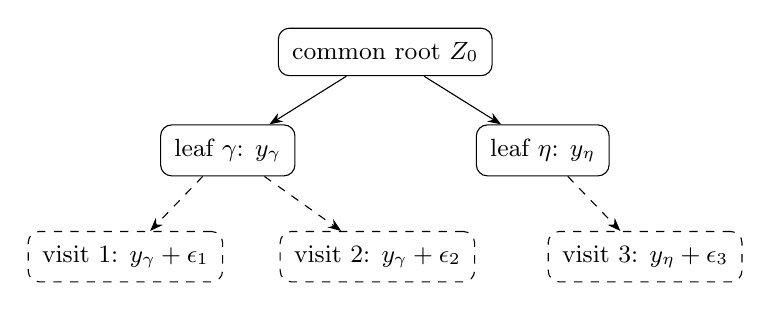
\begin{tikzpicture}[>=Stealth, every node/.style={font=\small},
                     shared/.style={draw,rounded corners,inner sep=5pt},
                     visit/.style={draw,dashed,rounded corners,inner sep=5pt}]
  \node[shared] (root) at (0,0) {common root $Z_0$};
  \node[shared] (left) at (-2,-1.25) {leaf $\gamma$: $y_\gamma$};
  \node[shared] (right) at (2,-1.25) {leaf $\eta$: $y_\eta$};
  \node[visit] (vone) at (-3.3,-2.6) {visit $1$: $y_\gamma+\epsilon_1$};
  \node[visit] (vtwo) at (-.1,-2.6) {visit $2$: $y_\gamma+\epsilon_2$};
  \node[visit] (vthree) at (3.3,-2.6) {visit $3$: $y_\eta+\epsilon_3$};
  \draw[->] (root)--(left);
  \draw[->] (root)--(right);
  \draw[->,dashed] (left)--(vone);
  \draw[->,dashed] (left)--(vtwo);
  \draw[->,dashed] (right)--(vthree);
 \end{tikzpicture}
 \caption{A two-leaf schematic of the Gaussian construction before
 reweighting. Shared increments
 belong to tree vertices, while residual noises belong to replica visits.
 The centered Gaussian residuals $\epsilon_1,\epsilon_2,\epsilon_3$ are
 independent and have variance $D-b_{k-1}$, even though visits $1$ and $2$
 have the same leaf label.}
 \label{arr:residual-figure}
\end{figure}

\subsection{Fresh Gaussian fields and passage through array limits}

\begin{lemma}[Bounded reweighting of convergent arrays]
\label{arr:limit}
Let a sequence of random base probabilities have jointly convergent
arrays of bounded observables and of the conditional covariances of
finitely many fresh centered Gaussian fields.  The fields are sampled
independently of the base probability conditional on its data, with any
specified independence between field components.  Then the following
averages converge, as determined by those limiting arrays:
\begin{enumerate}
 \item bounded continuous functions of the listed observable and field
 evaluations on finitely many base replicas;
 \item the same tests after reweighting by a fixed continuous function
 of the listed evaluations at one replica, bounded between two fixed
 positive constants;
 \item the expected logarithm of the normalizing integral of that factor.
\end{enumerate}
Independent finite-spin averages may be included.  The assertion remains
valid at singular limiting covariance matrices.  If the limiting
off-diagonal covariance entries are ordered functions of a scalar
ultrametric Ghirlanda--Guerra array, its evaluations can be obtained by
the quantized cascades of Lemma~\ref{arr:quantization}, retaining the true
diagonal variances and using \eqref{arr:residual-average}, provided the
base observables and tests used in the evaluation are also approximated
by these bins in probability on every finite replica restriction.  This
condition includes constants and continuous tests of the scalar overlap
and the quantized covariance coordinates.
\end{lemma}

\begin{proof}
On any fixed number of base replicas, the conditional joint Gaussian
law is a continuous function of its covariance matrix, also on the
boundary of the positive semidefinite cone.  For example, couple it as
$C^{1/2}g$; the nonnegative matrix square root is continuous and the
Gaussian vector $g$ has fixed dimension.  Bounded continuous tests
therefore pass to the joint array limit.

Write the positive reweighting factor as $A$, and let $Z=P(A)$ for the
base probability $P$.  If $0<c\leq A\leq C$, then $c\leq Z\leq C$.
An $r$-replica reweighted test has expectation
\[
 \mathbb E\left[
   Z^{-r}P^{\otimes r}\left(F\prod_{\ell=1}^r A_\ell\right)
 \right].
\]
Uniformly approximate $z^{-r}$ on $[c,C]$ by polynomials.  Each monomial
$Z^j$ is represented by $j$ additional base replicas, evaluated in the
same fresh fields.  The resulting terms are finite-replica tests covered
by the first part, and the uniform approximation controls the error.
Approximating $\log z$ on the same interval proves the logarithmic
assertion.  Finite-spin variables are simply additional independent base
variables in this argument.

Finally quantize all the ordered covariance coordinates jointly.  Their
finite-replica matrices converge by
Lemma~\ref{arr:quantization}, and the other observables and tests converge
by the additional approximation hypothesis.  Gaussian continuity and
the same polynomial argument therefore apply.  The shared Gaussian construction with
independent residuals has exactly those matrices, including on repeated
leaf visits.  Lemma~\ref{arr:cascade} identifies the quantized shape law,
and Lemma~\ref{arr:tilt} evaluates its bounded reweightings.  Unbounded
factors require an additional uniform-integrability argument; the cavity
calculation below supplies the particular truncation estimate it needs.
\end{proof}

\begin{lemma}[Evaluation of one fresh pattern]
\label{arr:fresh-pattern}
Suppose that the limiting spin-overlap array of a sequence of base Gibbs
probabilities has diagonal one, is Gram, and satisfies the
Ghirlanda--Guerra property.  Let $p$ be the quantile of its off-diagonal
two-replica law.  For a fresh independent Gaussian pattern field $g(x)$
with conditional covariance $R(x,x')$, and bounded continuous $f$,
\begin{equation}
 \lim\mathbb E\log\langle e^{f(g(x))}\rangle=V_f(p),
 \label{arr:fresh-pattern-value}
\end{equation}
whenever $V_f$ is understood through its continuous quantile extension.
In particular this applies to the smooth potentials used in the proof
before the final approximation step.
\end{lemma}

\begin{proof}
Theorem~\ref{arr:ultrametric} gives positivity and ultrametricity.
Lemma~\ref{arr:limit} passes the bounded positive factor through the array
limit.  Round the off-diagonal overlap into levels
$p_0\leq\cdots\leq p_{k-1}$ with probabilities $w_i$, leaving its
diagonal one.  On the corresponding cascade, first integrate the
independent variance $1-p_{k-1}$ at each visit.  The terminal shared-field
log factor is consequently
\[
 U_{k-1}(x)=\log\mathbb E
      e^{f(x+\sqrt{1-p_{k-1}}G)}.
\]
The remaining branch transforms have coefficients
$\zeta_{k-1},\ldots,\zeta_1$, by Lemma~\ref{arr:tilt}, and the common
root Gaussian is averaged with coefficient zero.  These are precisely
the defining transforms of $V_f$ on the rounded step quantile: its final
coefficient is one, and its initial coefficient is zero.  Sending the
rounding error to zero proves \eqref{arr:fresh-pattern-value}, by
Lemma~\ref{arr:limit} and continuity of the recursion in its quantile.
For bounded continuous $f$ this also supplies a direct description of
that extension: Lemma~\ref{arr:law-continuity} and the bounded reweighting
argument show that the cascade values have a unique continuous limit.
\end{proof}

\subsection{Gaussian Gibbs calculus and variance bounds}

\begin{lemma}[Gaussian differentiation]
\label{arr:calculus}
Let $P$ be a probability reference measure, possibly random but
independent of the Gaussian fields under consideration.  For independent
centered Gaussian energies with covariances $C_0,C_1$, interpolate using
$H_t=\sqrt{1-t}\,H_0+\sqrt t\,H_1$, and put
$\Delta=C_1-C_0$.  Then
\begin{equation}
 \frac{d}{dt}\mathbb E\log P(e^{H_t})
 =\frac12\mathbb E\langle\Delta_{11}-\Delta_{12}\rangle_t.
 \label{arr:gaussian-log-derivative}
\end{equation}
For a bounded $r$-replica test $F$ independent of these fields,
\begin{align}
 \frac{d}{dt}\mathbb E\langle F\rangle_t
 =\frac12\mathbb E\Bigg\langle F\Bigg(
 &\sum_{a,b=1}^r\Delta_{ab}
 -2r\sum_{a=1}^r\Delta_{a,r+1}\notag\\
 &+r(r+1)\Delta_{r+1,r+2}-r\Delta_{r+1,r+1}
 \Bigg)\Bigg\rangle_t,
 \label{arr:replica-derivative}
\end{align}
so its magnitude is at most
$(2r^2+r)\|F\|_\infty\|\Delta\|_\infty$.
If an independent centered Gaussian field $Y$ of covariance $C$ enters
the energy with coefficient $s$, Gaussian integration by parts also gives
\begin{equation}
 \mathbb E\langle Y(1)F\rangle
 =s\,\mathbb E\left\langle
  F\left(\sum_{a=1}^r C_{1a}-rC_{1,r+1}\right)
 \right\rangle.
 \label{arr:gaussian-insertion}
\end{equation}
These formulas hold for finite spin spaces with countably many cascade
labels whenever the covariances are bounded at the fixed system size.
They can be integrated up to the endpoints of covariance segments.
\end{lemma}

\begin{proof}
For finitely many states, differentiate the coupling $H_t$ and apply
ordinary Gaussian integration by parts.  This contracts one half of the
energy Hessian with $\Delta$.  A derivative of a normalized $r$-replica
integral inserts the sum over its $r$ sampled states minus $r$ times the
insertion at one extra replica.  A second derivative and contraction
give \eqref{arr:replica-derivative}; the sum of its absolute coefficients,
including the factor $1/2$, is $2r^2+r$.  The first derivative of the log
partition gives \eqref{arr:gaussian-log-derivative}, and a single
integration by parts gives \eqref{arr:gaussian-insertion}.

To pass to countable labels, truncate to increasing finite label sets
chosen independently of the added fields and renormalize their reference
weights.  Uniform integrability follows from elementary Gaussian moment
bounds.  For example, if a Gaussian energy has pointwise variance at most
$K$, then, conditionally on its independent probability reference,
\begin{equation}
 \mathbb E Z^p\leq e^{p^2K/2},\qquad
 \mathbb E Z^{-p}\leq e^{p^2K/2},\qquad
 Z=P(e^H),\quad p\geq1.
 \label{arr:partition-moments}
\end{equation}
The first inequality is Jensen's inequality for $x^p$; the second uses
$[P(e^H)]^{-p}\leq P(e^{-pH})$.  Cauchy--Schwarz and the same
single-state Gaussian moments control polynomial Gaussian insertions,
and exponentials of sums of absolute values of finitely many such
fields.  Thus Gibbs derivatives, their Gaussian insertions, and the
logarithms have uniformly integrable bounds on compact coefficient sets.
The truncated integrals converge almost surely and in the necessary
moments.  Bounded pattern log factors can be absorbed into the reference;
if estimates retain them explicitly, their exponential costs are
integrable for either a fixed count or an independent Poisson count.

Integrate the finite-state covariance derivative first and then pass to
the limit using its uniform bound.  Gaussian coupling and the same
moment bounds give continuity at segment endpoints.  Ordinary energy
parameter derivatives and \eqref{arr:gaussian-insertion} pass to the
limit by the polynomial-insertion bounds.  This proves the stated
extensions.
\end{proof}

\begin{lemma}[Elementary variance estimates]
\label{arr:variance}
A function of finite standard Gaussian data with Euclidean Lipschitz
constant $A$ has variance at most $A^2$.  A function of independent
inputs whose value changes by at most $c_i$ when input $i$ is replaced
has variance at most $\sum_i c_i^2$.  If a function $a$ on the integers
has Lipschitz constant $c$ and $K$ is Poisson with mean $\lambda$, then
$\operatorname{Var}(a(K))\leq c^2\lambda$.
\end{lemma}

\begin{proof}
For a smooth function of Gaussian data, interpolate two standard
Gaussian copies from independent to identical, with cross covariance
$tI$.  Gaussian integration by parts differentiates their product
expectation into the expectation of their gradient inner product.
Integrating from zero to one and using the gradient bound proves the
first claim.  Truncation and smoothing extend it to Lipschitz functions.
For the second, reveal the independent inputs successively and sum the
variances of the martingale differences, each bounded by $c_i^2$.
For the third, let $K'$ be an independent copy and use
\[
 \operatorname{Var}(a(K))
 =\tfrac12\mathbb E[(a(K)-a(K'))^2]
 \leq\tfrac{c^2}{2}\mathbb E[(K-K')^2]=c^2\lambda.
\]
\end{proof}

\section{The upper bound by enriched affine comparison}
\label{upper:section}

We continue to assume $f\in C_c^\infty(\mathbb R)$. The upper
bound uses a finite cascade as an additional Gibbs coordinate.
A Gaussian perturbation with vanishing pressure cost forces the joint
overlap identities at deterministic minimizers of a comparison functional.
The field derivatives at those minimizers give precisely the tail
order needed in Proposition~\ref{var:continuity-order}.
The comparison combines Gaussian interpolation in the tradition of
Guerra~\cite{guerra2003} with Mourrat's enriched supersolution
method~\cite[Section~4]{mourrat2021}. In particular, the use of penalized
deterministic contact points to obtain overlap identities follows the
strategy of that work. We give the estimates for the present model,
where Poisson differentiation of the pattern density replaces the
Gaussian interaction derivative.

\begin{proposition}[Upper bound]
\label{upper:bound}
For every nondecreasing $[0,1]$-valued path $q$,
\begin{equation}
\label{upper:conclusion}
 \limsup_{N\to\infty}\mathbb E p_N
 \le \alpha V_f(q)+S_{\mathrm I}(q).
\end{equation}
Consequently the limit superior is bounded above by the
variational infimum in Theorem~\ref{thm:main}.
\end{proposition}

\subsection{The enriched model and its finite-size estimates}

We use the cascade-field enrichment of Mourrat and
Panchenko~\cite{mourratpanchenko2020}: the cascade label is an additional
Gibbs coordinate, and a hierarchical Gaussian magnetic field probes the
spin overlap. The diagonal subtraction below uses the same normalization
principle. The nonlinear patterns act only on the spins.

Fix a step path $q$ on the partition
$0=\zeta_0<\cdots<\zeta_k=1$, with
$q_{k-1}<1$ and $S_{\mathrm I}(q)<\infty$.
Use the depth-$(k-1)$ cascade of Lemma~\ref{arr:cascade}, with
leaf weights $v_\gamma$ and common level $\gamma\wedge\eta$.
When $k=1$ the cascade has its single root leaf of weight one.
The reference probability on pairs $(x,\gamma)$ is
$\nu_N(dx)v_\gamma$. Define
\[
 R(x,x')=\frac{x\cdot x'}N,
 \qquad T(\gamma,\eta)=\frac{\gamma\wedge\eta}{k}.
\]
The array $T$ is positive semidefinite: assign independent
Gaussian increments of variance $1/k$ to each edge of the tree
and sum them along each root-to-leaf path. The covariance of
these sums is $T$. Its diagonal is $(k-1)/k$, including the
value zero for $k=1$.

Let $0\le t\le\alpha$ and let $K$ be Poisson with mean $Nt$.
The $K$ independent Gaussian patterns act only on $x$. For a
field path $0\le h_0\le\cdots\le h_{k-1}$, add the energy
\[
 z(\gamma)\cdot x-\frac N2h_{k-1},
\]
where the $N$ coordinates of $z$ are independent centered
Gaussian fields on the cascade, each with covariance
$h_{\gamma\wedge\eta}$. They are constructed from common root
increments of variance $h_0$ and independent vertex increments
of variances $h_i-h_{i-1}$ thereafter.

Enumerate the monomials
\[
 \kappa_j(R,T)=R^pT^d,
 \qquad p,d\in\{0,1,2,\ldots\},\quad p+d\ge1,
\]
so that every such monomial has a fixed finite index $j$.
The convention is $T^0=1$, also when $T=0$.
There are independent centered Gaussian fields $Y_j(x,\gamma)$
with these covariances. One explicit construction uses a standard
Gaussian tensor contracted with $(x/\sqrt N)^{\otimes p}$
to produce covariance $R^p$ (a scalar Gaussian for $p=0$).
For $d>0$, place independent copies at the vertices and multiply
them by square roots of the increments of $(i/k)^d$; for
$d=0$ use just a common root copy. The resulting covariance is
the indicated product. This also covers identically zero
covariances without exception.

All these fields are independent of the patterns and the field
$z$. Set
\begin{equation}
\label{upper:perturbation}
 e_N=N^{-1/16},\qquad
 \sqrt N e_N\sum_{j=1}^N2^{-j}u_jY_j(x,\gamma),
 \qquad 1\le u_j\le2,
\end{equation}
and add this perturbation to the energy. Denote the random
pressure of the resulting model by $P_N(t,h,u)$ and put
\begin{equation}
\label{upper:F}
 F_N(t,h,u)=-\mathbb E P_N(t,h,u).
\end{equation}
Every parameter is held deterministic in this expectation.
The diagonal and the absolute value of every covariance
$\kappa_j$ are at most one, so the perturbation covariance is
bounded by $CNe_N^2$. Lemma~\ref{arr:calculus} therefore shows
that turning the perturbation on or off changes the expected
pressure by at most $Ce_N^2$, uniformly in these parameters.
At the energy scale, however, the coefficient of each fixed $Y_j$
grows like $\sqrt N e_N=N^{7/16}$; this is the scale against
which its fluctuations will be compared.

At $t=0$ with the perturbation removed, spin integration at a
leaf gives the product $\prod_{a=1}^N\cosh z_a(\gamma)$.
The independent-coordinate form of Lemma~\ref{arr:tilt} and
the diagonal subtraction imply
\begin{equation}
\label{upper:initial-value}
 \mathbb E P_N(0,h,\text{no perturbation})=\ell(h).
\end{equation}
With patterns and perturbations present, one can instead apply
that lemma to the complete spin log integral at each leaf.
Conditional on patterns, count, and common root Gaussian data,
the remaining vertex marks have exactly the conditional
independence required there. Hence the sampled label shape has
the original cascade law. In particular, for every $N,t,h,u$,
\begin{equation}
\label{upper:label-law}
 \mathbb E\langle\mathbf 1_{
        \{\gamma^1\wedge\gamma^2=i\}}\rangle=w_i.
\end{equation}

\begin{lemma}[Uniform concentration on a field cap]
\label{upper:concentration}
For each fixed $H<\infty$ there is a constant $C_H$, also
depending on the fixed partition, $\alpha$, and $f$, such that
\begin{equation}
\label{upper:variance}
 \operatorname{Var}(P_N(t,h,u))\le\frac{C_H}{N}
\end{equation}
whenever $0\le t\le\alpha$, $0\le h_0\le\cdots\le
h_{k-1}\le H$, and $u\in[1,2]^N$.
\end{lemma}

\begin{proof}
Write $L_N=NP_N$. Put the patterns, their count, and all common
root Gaussian variables into the root data. Apply
Lemma~\ref{arr:tilt} to the leaf spin log integral. If $X_0$
is the resulting recursion value at the root, that lemma gives
\[
 \mathbb E[L_N\mid\text{root data}]=X_0,
 \qquad
 \mathbb E[(L_N-X_0)^2\mid\text{root data}]\le C_{\zeta}.
\]
The second assertion can also be seen directly: $L_N-X_0$
is the difference between the logarithms of the transformed
and original unnormalized cascade totals. Each total has the
original conditional law, whose logarithm has finite second
moment depending only on the fixed cascade. The two totals
need not be independent for this bound.

Conditional on $K$, the norm of the coefficient vector of the
common Gaussian variables in the energy at any fixed state is
at most $C_H\sqrt N$. Indeed its squared norm is the sum of
the common variances, bounded by $NH+CNe_N^2$.
The spin log integral has the same Lipschitz constant in these
variables: the difference of two log integrals is bounded by
the supremum of the difference of their energies. Every
subsequent log-exponential transform preserves such a uniform
change bound. Thus $X_0$ has Gaussian variance at most $C_HN$
by Lemma~\ref{arr:variance}. Replacing one of the $K$ patterns
changes $X_0$ by at most $2\|f\|_\infty$, because this bound
holds for every leaf energy and is preserved by each recursion.
The independent-input variance bound therefore adds at most
$C K$. Combining these independent blocks gives
\[
 \operatorname{Var}(X_0\mid K)\le C_HN+C K.
\]
The conditional mean $\mathbb E[X_0\mid K=m]$ changes by at
most $\|f\|_\infty$ between $m$ and $m+1$, by adding one
pattern under a coupling. If $K'$ is an independent copy,
the independent-copy variance formula bounds the variance of
this conditional mean by
$\|f\|_\infty^2\mathbb E(K-K')^2/2
=\|f\|_\infty^2Nt$.
The total variance of $L_N$ is consequently $O_H(N)$.
Division by $N^2$ proves \eqref{upper:variance}.
\end{proof}

\begin{lemma}[Derivatives of the comparison function]
\label{upper:derivatives}
The function $F_N$ is continuous on the parameter region above.
For every nonnegative nondecreasing direction $\lambda$ on
the fixed partition, its right directional derivative in $h$ is
\begin{equation}
\label{upper:field-derivative}
 \partial_{h,\lambda}F_N
 =\frac12\mathbb E\langle
       R_{12}\lambda_{\gamma^1\wedge\gamma^2}\rangle.
\end{equation}
For $t>0$, its time derivative is
\begin{equation}
\label{upper:time-derivative}
 \partial_tF_N
 =-\mathbb E\log\left\langle
    \exp f(\widehat g\cdot x/\sqrt N)\right\rangle,
\end{equation}
where $\widehat g$ is an independent standard Gaussian pattern.
\end{lemma}

\begin{proof}
Increasing $h$ by $a\lambda$ adds an independent Gaussian
energy with covariance
\[
 aN R(x,x')\lambda_{\gamma\wedge\eta}.
\]
It also changes the deterministic subtraction by
$-aN\lambda_{k-1}/2$.
The diagonal covariance term in Lemma~\ref{arr:calculus}
cancels this subtraction, proving
\eqref{upper:field-derivative} after reversing the pressure
sign. Poisson differentiation gives
\[
 \frac{d}{dt}\mathbb E L_N(K)
 =N\mathbb E[L_N(K+1)-L_N(K)],
\]
whose increment is the logarithm in
\eqref{upper:time-derivative}. Its absolute value is bounded
by $\|f\|_\infty$, so differentiating the Poisson series
and passing to its limits are justified. Continuity in $t$
follows also by coupling Poisson counts. Continuity in $h$
follows by coupling the vertex increments and the Gaussian
interpolation estimates, including at zero increments;
continuity in $u$ follows from ordinary Gaussian-coupling
differentiation. The countable label set is handled by the
field-independent finite truncations and moment bounds in
Lemma~\ref{arr:calculus}.
\end{proof}

\subsection{Deterministic minimizers and their overlap identities}

The quadratic penalty and concentration argument at the minimizing
parameters implement the contact-point construction in
Mourrat~\cite[Section~4, in particular equations~(4.19)--(4.28)]{mourrat2021}.
The proof is included because the pattern contribution and its
concentration estimates differ from those of the Gaussian bipartite
Hamiltonian treated there.

Suppose, contrary to the step version of
\eqref{upper:conclusion}, that for some $\eta>0$ and an
infinite sequence of dimensions,
\[
 \mathbb E p_N\ge S_{\mathrm I}(q)+\alpha V_f(q)+\eta.
\]
Couple $\lfloor\alpha N\rfloor$ patterns to a Poisson count
of mean $N\alpha$ by using the same initial rows. The pressure
change in expectation is at most
\[
 \frac{\|f\|_\infty}{N}
 \mathbb E|K-\lfloor\alpha N\rfloor|=O(N^{-1/2}).
\]
Choose $\delta>0$ with $\alpha\delta<\eta/4$. On the
compact parameter region
\[
 0\le t\le\alpha,\quad
 0\le h_0\le\cdots\le h_{k-1}\le H,\quad
 u\in[1,2]^N,
\]
minimize the continuous function
\begin{equation}
\label{upper:objective}
 \begin{split}
 J_N(t,h,u)={}&F_N(t,h,u)
       -\frac12\sum_{i=0}^{k-1}w_iq_ih_i
       +S_{\mathrm I}(q)+t\{V_f(q)+\delta\}\\
       &+\sum_{j=1}^N2^{-j}(u_j-3/2)^2.
 \end{split}
\end{equation}
The fixed field cap $H$ will now be chosen.

\begin{lemma}[The field cap is coercive]
\label{upper:coercive}
For the fixed partition,
\begin{equation}
\label{upper:field-growth}
 \ell(h)\le (\mathbb E|G|)\sqrt{h_0}+C_{\zeta}
                   -\frac12\sum_{i=0}^{k-1}w_ih_i.
\end{equation}
For sufficiently large fixed $H$, every sufficiently large
dimension in the violating sequence has a minimizer of
\eqref{upper:objective} satisfying
$t>0$ and $h_{k-1}<H$.
\end{lemma}

\begin{proof}
Start from $\log\cosh x\le|x|$. For $d>0$,
\[
 \mathcal T_{s,d}(|\cdot|+c)(x)
 \le |x|+c+\frac{ds}{2}+\frac{\log2}{d},
\]
because $e^{d|x+\sqrt sG|}\le
e^{d(x+\sqrt sG)}+e^{-d(x+\sqrt sG)}
\le e^{d|x|}(e^{d\sqrt sG}+e^{-d\sqrt sG})$ after
taking expectations. Propagate this bound through levels
$k-1,\ldots,1$ and then average $|\sqrt{h_0}G|$ at the
root. The variance-dependent constant is
\[
 -\frac{h_{k-1}}2
 +\frac12\sum_{i=1}^{k-1}\zeta_i(h_i-h_{i-1})
 =-\frac12\sum_{i=0}^{k-1}w_ih_i,
\]
which proves \eqref{upper:field-growth}, with
$C_\zeta=\sum_{i=1}^{k-1}(\log2)/\zeta_i$; the sum is
zero if $k=1$.

Adding the patterns changes pressure by at most
$\alpha\|f\|_\infty$ in expectation, and the perturbation
cost is $O(e_N^2)$. Thus
\[
 F_N(t,h,u)\ge-\ell(h)-\alpha\|f\|_\infty-O(e_N^2).
\]
Since $S_{\mathrm I}(q)\ge0$, $|V_f(q)|\le\|f\|_\infty$,
and the quadratic penalty is nonnegative, on $h_{k-1}=H$
this gives the uniform lower bound
\begin{equation}
\label{upper:cap-bound}
 J_N(t,h,u)\ge
 \frac{w_{k-1}(1-q_{k-1})}{2}H
 -(\mathbb E|G|)\sqrt H-C_\zeta
 -2\alpha\|f\|_\infty-O(e_N^2).
\end{equation}
The linear coefficient is strictly positive, so choose $H$
large enough that this lower bound is positive for all large
$N$. At $t=0$, the entropy definition and
\eqref{upper:initial-value} instead give
$J_N(0,h,u)\ge-O(e_N^2)$.
Finally, testing $t=\alpha$, $h=0$, and $u_j=3/2$ gives
$J_N\le-\eta/2$ for all sufficiently large dimensions in
the violating sequence, by the Poisson coupling, the choice
of $\delta$, and the perturbation bound. Hence a minimizing
triple lies on neither of the excluded faces.
\end{proof}

Choose a deterministic minimizing triple $(t_N,h_N,u_N)$
for each such dimension. Comparing it with the same $(t_N,h_N)$
and all $u_j=3/2$ shows that
\begin{equation}
\label{upper:penalty}
 \sum_{j=1}^N2^{-j}(u_{N,j}-3/2)^2=O(e_N^2),
 \qquad u_{N,j}=3/2+O_j(e_N)\quad\text{for fixed }j.
\end{equation}
Indeed any two allowed perturbations have expected pressures
within $O(e_N^2)$ of the unperturbed model. In particular,
each fixed coordinate of $u_N$ is eventually interior.

\begin{lemma}[Joint identities at deterministic minimizers]
\label{upper:gg}
Every subsequential limit of the sampled joint arrays $(R,T)$
at these deterministic minimizing triples satisfies the joint
Ghirlanda--Guerra identities of Definition~\ref{arr:gg}.
\end{lemma}

\begin{proof}
Fix $j$. All derivatives in this proof hold $(t_N,h_N)$ and
the other perturbation coordinates fixed. Abbreviate
$a_{N,j}=\sqrt N e_N2^{-j}$ and
$g(v)=\mathbb E P_N(t_N,h_N,u_1,\ldots,v,\ldots,u_N)$.
Ordinary Gibbs differentiation gives
\begin{align}
\label{upper:u-derivatives}
 \partial_{u_j}P_N&=\frac{e_N2^{-j}}{\sqrt N}
                         \langle Y_j\rangle,\\
 g''(u_{N,j})&=e_N^24^{-j}
   \mathbb E\langle(Y_j-\langle Y_j\rangle)^2\rangle.
\end{align}
The random function $P_N$ is convex in $u_j$, since it is
a log integral of an energy affine in that coordinate.
We first control the Gibbs fluctuation of $Y_j$ around
$\langle Y_j\rangle$ by the curvature at the minimum. We then
control the disorder fluctuation of $\langle Y_j\rangle$ by
finite differences. Both estimates hold at the chosen deterministic
coordinate $u_{N,j}$, without averaging it.

Interior minimality of $J_N$ implies
$g'(u_{N,j})=2\cdot2^{-j}(u_{N,j}-3/2)$ and
$g''(u_{N,j})\le2\cdot2^{-j}$. Consequently
\begin{equation}
\label{upper:thermal}
 \mathbb E\langle|Y_j-\langle Y_j\rangle|\rangle
 \le C_j e_N^{-1}.
\end{equation}
For the disorder fluctuation, use minimality over an interval
around $u_{N,j}$. Cancellation of the linear term gives
\begin{equation}
\label{upper:taylor}
 0\le g(u_{N,j}\pm s)-g(u_{N,j})
           \mp s g'(u_{N,j})\le2^{-j}s^2
\end{equation}
whenever both displaced coordinates lie in $[1,2]$.
The first inequality uses convexity of $g$.

For any differentiable convex random function, its derivative
at a point lies between the backward and forward difference
quotients. Apply this fact to $P_N$ with step $s$, and subtract
$g'(u_{N,j})$. The mean quotient errors are at most $2^{-j}s$
by \eqref{upper:taylor}. Replacing each of the three random
function values by its expectation costs at most
$C_H/(s\sqrt N)$ in $L^1$, by
Lemma~\ref{upper:concentration}. Taking the positive and
negative parts therefore yields
\begin{equation}
\label{upper:derivative-fluctuation}
 \mathbb E|\partial_{u_j}P_N-g'(u_{N,j})|
 \le C_js+\frac{C_H}{s\sqrt N}.
\end{equation}
By \eqref{upper:penalty}, $s=N^{-1/4}$ is eventually allowed.
Then the right side is $O_j(N^{-1/4})=o(e_N^2)$.
Multiplying by $\sqrt N/(e_N2^{-j})$ in
\eqref{upper:u-derivatives}, and adding
\eqref{upper:thermal}, gives
\begin{equation}
\label{upper:Y-concentration}
 \mathbb E\langle|Y_j-\mathbb E\langle Y_j\rangle|\rangle
 =o(\sqrt N e_N).
\end{equation}
Explicitly, the two contributions are
$O_j(N^{1/16})$ and $O_j(N^{5/16})$, whereas
$\sqrt N e_N=N^{7/16}$. All assertions concern one fixed
$j$ at a time; no bound uniform in $j\le N$ is needed.

Let $D$ be a bounded continuous function of the first
$n\times n$ joint overlap block, $n\ge2$. Gaussian
integration by parts in the field $Y_j$ gives
\begin{equation}
\label{upper:ibp}
 \mathbb E\langle Y_j(1)D\rangle
 =a_{N,j}u_{N,j}\,
 \mathbb E\left\langle D\left(
    \sum_{l=1}^n\kappa_j(R_{1l},T_{1l})
       -n\kappa_j(R_{1,n+1},T_{1,n+1})\right)\right\rangle.
\end{equation}
The overlap test has no direct dependence on the Gaussian
coordinates of $Y_j$, so Lemma~\ref{arr:calculus} applies.
By \eqref{upper:Y-concentration}, the left side equals
$\mathbb E\langle Y_j\rangle\mathbb E\langle D\rangle
+o(\sqrt N e_N)$. The single-replica version of
\eqref{upper:ibp} reads
\[
 \mathbb E\langle Y_j\rangle
 =a_{N,j}u_{N,j}
   \{\kappa_j(1,(k-1)/k)
          -\mathbb E\langle\kappa_j(R_{12},T_{12})\rangle\}.
\]
Substitute this expression and cancel the constant diagonal.
After division by $n a_{N,j}u_{N,j}$, one obtains
\begin{align*}
 \mathbb E\langle D\kappa_j(R_{1,n+1},T_{1,n+1})\rangle
 ={}&\frac1n\mathbb E\langle D\rangle
             \mathbb E\langle\kappa_j(R_{12},T_{12})\rangle\\
 &+\frac1n\sum_{l=2}^n
       \mathbb E\langle D\kappa_j(R_{1l},T_{1l})\rangle+o(1).
\end{align*}
Pass to a joint array subsequence, which exists because the
entries range over a compact set. The identity holds for every
fixed monomial and hence, by linearity and uniform polynomial
approximation, for every continuous function of a pair $(R,T)$.
Continuous tests of the finite block determine its measures,
so the same identities hold with every bounded measurable
block test. This is the full conditional-law formulation in
Definition~\ref{arr:gg}.
\end{proof}

\subsection{Ordered supports and the derivative contradiction}

The no-crossing argument below is the monotone-coupling mechanism in
spin-glass synchronization; compare Panchenko~\cite[Section~4, Lemma~2]{panchenko2015multispecies}.
Its input here is the joint identity already proved for the spin and tree
overlaps.

\begin{lemma}[Ordered coupling of the spin and tree overlaps]
\label{upper:synchronization}
In any joint array limit from Lemma~\ref{upper:gg}, the
two-replica law of $(R_{12},T_{12})$ is supported on a set
ordered in both coordinates. If $p$ is the quantile of
$R_{12}$, the conditional law of $R_{12}$ given $T_{12}=i/k$
is the law of $p(U)$ for $U$ uniform on
$(\zeta_i,\zeta_{i+1})$.
\end{lemma}

\begin{proof}
The arrays $R$ and $R+T$ are Gram arrays of constant diagonal,
and their scalar identities follow from the joint identities.
Theorem~\ref{arr:ultrametric} therefore makes both arrays
ultrametric and makes the off-diagonal entries of $R$
nonnegative. They are at most one by its Gram diagonal.
The tree array $T$ is already ultrametric.

Suppose the two-replica support contained two strictly crossed
points. Choose small neighborhoods $A,B$ of these points so
that every $(r,t)\in A$ and $(r',t')\in B$ satisfy
$r<r'$ and $t>t'$. Both neighborhoods have positive
two-replica probability. The joint conditional law with
$n=2$ then gives
\[
 \mathbb P\big((R_{12},T_{12})\in A,
               (R_{13},T_{13})\in B\big)
 \ge\tfrac12\mathbb P((R_{12},T_{12})\in A)
              \mathbb P((R_{12},T_{12})\in B)>0.
\]
On this event, ultrametricity of $R$ forces $R_{23}=R_{12}$:
the inequalities for edges $12$ and $23$ give the two opposite
inequalities once $R_{12}<R_{13}$ is used. Likewise,
ultrametricity of $T$ forces $T_{23}=T_{13}$.
It follows that $R_{23}+T_{23}$ is strictly smaller than both
$R_{12}+T_{12}$ and $R_{13}+T_{13}$, contradicting
ultrametricity of $R+T$. Hence such support points cannot
exist.

By \eqref{upper:label-law}, the successive values $i/k$ of
$T_{12}$ have masses $w_i$. The conditional spin-overlap
supports at these levels are ordered: every value at an
earlier level is at most every value at a later level.
Thus sorting their mixture simply concatenates these
conditional laws in blocks of lengths $w_i$. This is exactly
the claimed quantile description, including any atoms shared
by adjacent conditional supports.
\end{proof}

The ordered conditional laws identify field directional derivatives with
weighted block averages of the spin-overlap quantile. Directions that
select a tail of the partition give the comparisons required by
Proposition~\ref{var:continuity-order}.

\begin{proof}[Proof of Proposition~\ref{upper:bound}]
Continue along the violating sequence and its minimizing
triples. Extract a joint array limit and let $p$ be the
spin-overlap quantile given by
Lemma~\ref{upper:synchronization}. For any nonnegative
nondecreasing step direction $\lambda$ on the fixed
partition, sufficiently small positive displacements of $h_N$
are feasible, since $h_{N,k-1}<H$. Minimality and
\eqref{upper:field-derivative} yield
\[
 \mathbb E\langle R_{12}
                  \lambda_{\gamma^1\wedge\gamma^2}\rangle
 \ge\sum_{i=0}^{k-1}w_iq_i\lambda_i.
\]
Pass to the joint array limit and use its ordered conditional
laws to obtain
\begin{equation}
\label{upper:cone-inequality}
 \int_0^1p(u)\lambda(u)\,du
 \ge\int_0^1q(u)\lambda(u)\,du.
\end{equation}
Choose successively $\lambda_i=\mathbf 1_{\{i\ge j\}}$,
$0\le j\le k-1$. This gives
\[
 \int_{\zeta_j}^1p(u)\,du
 \ge\int_{\zeta_j}^1q(u)\,du
 \qquad(0\le j\le k),
\]
where $j=k$ is equality. The function
$s\mapsto\int_s^1p(u)\,du$ is concave, because its
almost-everywhere derivative is the nonincreasing function
$-p(s)$. On each partition interval the corresponding tail
integral of $q$ is affine. Concavity places the first tail
above the chord joining its endpoint values, which in turn
lies above the second tail. Therefore the tail inequalities
hold for every $s\in[0,1]$. By
Proposition~\ref{var:continuity-order},
\begin{equation}
\label{upper:V-comparison}
 V_f(p)\le V_f(q).
\end{equation}

At every minimizing triple $t_N>0$, a small displacement to
the left in time is feasible, even if $t_N=\alpha$ or
$t_N\downarrow0$. Thus the derivative of $J_N$ with respect
to $t$ at that triple is nonpositive. On the other hand, the
fresh pattern in \eqref{upper:time-derivative} has covariance
$R$ and diagonal one. Lemma~\ref{arr:fresh-pattern}, applied
to the marginal limiting spin-overlap array, gives
\[
 \partial_t J_N(t_N,h_N,u_N)
 \longrightarrow -V_f(p)+V_f(q)+\delta\ge\delta>0.
\]
This contradicts the required sign at the minimizers and
proves \eqref{upper:conclusion} for every step trial with
$q_{k-1}<1$ and finite entropy. Infinite-entropy trials give
no restriction. Taking the infimum over finite step trials
and using Corollary~\ref{var:step-reduction} proves the
claimed bound for the full variational infimum, and hence
for every admissible $q$.
\end{proof}

\section{The perturbed bulk and restoration of two patterns}
\label{bulk:section}

Throughout this section and Section~\ref{cav:section}, fix
$f\in C_c^\infty(\mathbb R)$ and use the fixed pattern count
$M_N=\lfloor\alpha N\rfloor$.  All constants may depend on $f$ and
$\alpha$.  A further dependence on a fixed cavity size $L$ will be indicated.
For each $1\le j\le N$, let $Y_j$ be a centered Gaussian field on the
hypercube with covariance
\[
 \mathbb E Y_j(x)Y_j(x')=R(x,x')^j.
\]
Such a field is obtained by contracting an independent standard Gaussian
$j$-tensor with $(x/\sqrt N)^{\otimes j}$.  The fields are independent of
one another and of all patterns.  For a deterministic parameter sequence
$v=(v_j)_{j\ge1}\in[1,2]^{\mathbb N}$, add the energy
\begin{equation}\label{bulk:perturbation}
 H_N^v(x)=s_N\sum_{j=1}^N2^{-j}v_jY_j(x),
 \qquad s_N=N^{3/8},
 \qquad \xi_N^v(r)=\sum_{j=1}^N4^{-j}v_j^2r^j.
\end{equation}
Its covariance is $s_N^2\xi_N^v(R)$.  Let $Z_N^v$ be the resulting
partition function with probability prior $\nu_N$, and let $G_N^v$ be its
Gibbs probability.  Except when a parameter integral is displayed, every
expectation keeps $v$ fixed.  Write $\pi$ for product uniform probability
on $[1,2]^{\mathbb N}$ and set
\begin{equation}\label{bulk:averaged-free-energy}
 \mathcal F_N=\int\mathbb E\log Z_N^v\,\pi(dv).
\end{equation}
Because $\sup_{N,v,|r|\le1}|\xi_N^v(r)|<\infty$, covariance interpolation
from Lemma~\ref{arr:calculus} gives, uniformly in $v$,
\begin{equation}\label{bulk:perturbation-cost}
 \big|\mathbb E\log Z_N^v-N\mathbb E p_N\big|
 \le C s_N^2=C N^{3/4}.
\end{equation}
In particular $\mathcal F_N/N-\mathbb E p_N=O(N^{-1/4})$.

The next section expands the energy after adding $L$ spin coordinates.
The Gaussian field acting on each new coordinate has the empirical
covariance $B_N$ below; the mean quadratic term and the rescaling of
the old pattern arguments together contribute $LC_N/2$:
\begin{align}
 B_N(x,x')&=\frac1N\sum_{a=1}^{M_N}
                f'(b_a(x))f'(b_a(x')), \label{bulk:B}\\
 C_N(x)&=\frac1N\sum_{a=1}^{M_N}
           \bigl(f''(b_a(x))-b_a(x)f'(b_a(x))\bigr).           \label{bulk:C}
\end{align}
We will sample these observables from the full perturbed probability
$G_N^v$.  Compact support makes both uniformly bounded.  The kernel
$B_N$ is positive semidefinite, but its diagonal and $C_N$ need not be
constant at finite $N$.  Our task is to show that in every suitable
array limit the off-diagonal covariance is a deterministic
nondecreasing function of the spin overlap, while the diagonal and
$C_N$ are deterministic constants.

\subsection{Uniform good parameters for the omitted system}

To identify these limits, we need both first and second moments of the
empirical row averages.  One restored pattern will determine their
conditional means; two independently restored patterns will determine
the corresponding squares and eliminate the remaining variance.
Delete the last two patterns, retaining precisely the perturbation
\eqref{bulk:perturbation}, and denote the resulting Gibbs expectation by
$\langle\cdot\rangle_\circ$.  This definition is used for all sufficiently
large $N$ that $M_N\ge2$.

\begin{lemma}[Overlap identities on uniform good parameter sets]
\label{bulk:good-parameters}
There are measurable sets $\mathcal G_N\subset[1,2]^{\mathbb N}$ with
$\pi(\mathcal G_N)\to1$ such that the following holds.  For every
deterministic sequence $v(N)\in\mathcal G_N$, every subsequential limit
of the omitted system's sampled overlap array satisfies the
Ghirlanda--Guerra identities of Definition~\ref{arr:gg}.
\end{lemma}

\begin{proof}
Let $P_N^\circ$ be the omitted system's random normalized log partition
function.  Uniformly when each parameter lies in $[1/2,5/2]$, we have
\begin{equation}\label{bulk:concentration}
 \operatorname{Var}(P_N^\circ)\le \frac C N.
\end{equation}
Indeed, replacing one pattern changes its unnormalized log partition
function by at most $2\|f\|_\infty$.  Conditional on the patterns, its
Lipschitz constant in the independent Gaussian tensors defining the
perturbation is at most
$s_N(\sum_j4^{-j}v_j^2)^{1/2}\le Cs_N$.
The conditional Gaussian variance bound and the bounded-difference
bound for the conditional mean therefore give
$\operatorname{Var}(\log Z_N^\circ)\le C(N+s_N^2)\le CN$.
Both bounds are instances of Lemma~\ref{arr:variance}.

Fix $j$, with $N\ge j$, and put $t_j=s_N2^{-j}$.  Finite-dimensional
Gaussian integration by parts and differentiation of the spin sum give
\begin{align}
 \partial_{v_j}P_N^\circ
   &=\frac{t_j}{N}\langle Y_j\rangle_\circ,
   \label{bulk:parameter-derivative}\\
 \partial_{v_j}\mathbb E P_N^\circ
   &=\frac{t_j^2v_j}{N}
       \bigl(1-\mathbb E\langle R_{12}^j\rangle_\circ\bigr),
   \label{bulk:mean-derivative}\\
 \partial_{v_j}^2\mathbb E P_N^\circ
   &=\frac{t_j^2}{N}\mathbb E
      \big\langle(Y_j-\langle Y_j\rangle_\circ)^2\big\rangle_\circ.
   \label{bulk:thermal-derivative}
\end{align}
These operations are legitimate since the state space is finite and
Gaussian exponential moments control all derivatives on a compact
parameter interval.  Formula~\eqref{bulk:mean-derivative} is bounded in
absolute value by $Ct_j^2/N$ on the enlarged interval.  Integrating
\eqref{bulk:thermal-derivative} from $1$ to $2$ consequently yields
\begin{equation}\label{bulk:thermal-integral}
 \int_1^2\mathbb E
 \big\langle(Y_j-\langle Y_j\rangle_\circ)^2\big\rangle_\circ\,dv_j
 \le C.
\end{equation}
The other parameters remain arbitrary throughout this estimate.

For completeness, the concentration estimate needed for the quenched
mean of $Y_j$ follows from integrated convexity, without selecting a
parameter in advance.  Let $F=\mathbb E P_N^\circ$ and
$0<\eta<1/4$.  The forward and backward difference quotients bracket
$\partial_{v_j}P_N^\circ$.  Replacing each random function value in these
quotients by its expectation costs at most $C/(\eta\sqrt N)$ in
expected absolute value, by \eqref{bulk:concentration}.  For the mean
function, the forward error is bounded by
$F'(v_j+\eta)-F'(v_j)$, and the backward error by
$F'(v_j)-F'(v_j-\eta)$.  Integrating these differences over $[1,2]$
leaves intervals of total length at most $4\eta$ at the ends.  Since
$F'$ is bounded by $Ct_j^2/N$, this proves
\begin{equation}\label{bulk:convex-fluctuation}
 \int_1^2\mathbb E
 \big|\partial_{v_j}P_N^\circ-\partial_{v_j}\mathbb E P_N^\circ\big|
 \,dv_j
 \le C_j\eta\frac{s_N^2}{N}+\frac{C}{\eta\sqrt N}.
\end{equation}
Choose $\eta=N^{-1/8}$.  Both terms are $O_j(N^{-3/8})$, whereas
$s_N^2/N=N^{-1/4}$.  Combining
\eqref{bulk:parameter-derivative}, \eqref{bulk:thermal-integral}, and
Cauchy--Schwarz gives
\begin{align}
 &\int\mathbb E\big\langle
       |Y_j-\mathbb E\langle Y_j\rangle_\circ|
     \big\rangle_\circ\,\pi(dv) \nonumber\\
 &\qquad\le C+\frac{N}{t_j}\,O_j(N^{-3/8})
   =O_j(N^{1/4})=o(s_N).
 \label{bulk:integrated-deviation}
\end{align}
Here and below $j$ is fixed before $N\to\infty$.

Set
\[
 a_{j,N}(v)=s_N^{-1}\mathbb E\big\langle
   |Y_j-\mathbb E\langle Y_j\rangle_\circ|
 \big\rangle_\circ.
\]
By \eqref{bulk:integrated-deviation}, choose integers $J_N\le N$
increasing to infinity sufficiently slowly that
\[
 e_N:=\sum_{j\le J_N}\int a_{j,N}\,d\pi\longrightarrow0.
\]
With $\delta_N=\sqrt{e_N}+N^{-1}$, define
\[
 \mathcal G_N=\left\{v:\sum_{j\le J_N}a_{j,N}(v)\le\delta_N\right\}.
\]
Markov's inequality gives
$\pi(\mathcal G_N^c)\le e_N/\delta_N\to0$, and each fixed
$a_{j,N}$ tends to zero uniformly on $\mathcal G_N$.

To obtain the identities, let $D$ be a bounded continuous test of the
first $n\times n$ overlap block, $n\ge2$.  Integration by parts gives
\[
 \mathbb E\langle Y_j(x^1)D\rangle_\circ
 =t_jv_j\mathbb E\left\langle D\left(
       \sum_{l=1}^nR_{1l}^j-nR_{1,n+1}^j\right)\right\rangle_\circ.
\]
The left side differs from
$\mathbb E\langle Y_j\rangle_\circ\,\mathbb E\langle D\rangle_\circ$
by at most $\|D\|_\infty s_Na_{j,N}(v)$.  Using the corresponding
one-replica integration-by-parts identity and $R_{11}=1$ therefore gives
\begin{align*}
 &\mathbb E\langle D R_{1,n+1}^j\rangle_\circ
 -\frac1n\mathbb E\langle D\rangle_\circ
             \mathbb E\langle R_{12}^j\rangle_\circ
 -\frac1n\sum_{l=2}^n\mathbb E\langle D R_{1l}^j\rangle_\circ
 =o(1),
\end{align*}
uniformly on $\mathcal G_N$ for each fixed $j,n,D$.  Polynomial
approximation on $[-1,1]$, followed by determination of finite measures
by continuous tests, gives the full identities in every array limit.
This proves the stated quantifier for arbitrary deterministic choices
from the good sets.
\end{proof}

\subsection{Restored gradient covariances}

\begin{proposition}[Deterministic covariance and cavity correction]
\label{bulk:restoration}
Start with any deterministic good parameter sequence, on any subsequence
of dimensions.  Pass to a further subsequence on which the omitted
overlap array converges and the full system's joint sampled arrays
$(R_{lm},B_N(x^l,x^m),C_N(x^l))$ converge.  Let $\mu$ be the omitted
limit's two-replica overlap law.  The full limiting overlap array has the
same law as the omitted one.  There are deterministic constants
$a_{\mathrm d},c$ and a deterministic nondecreasing function $a$, defined
on a $\mu$-full ordered subset of $[0,1]$, such that almost surely
\begin{equation}\label{bulk:deterministic-covariances}
 B_{lm}=a(R_{lm})\quad(l\ne m),\qquad
 B_{ll}=a_{\mathrm d},\qquad C_l=c,
 \qquad 0\le a\le a_{\mathrm d}\le\alpha\|f'\|_\infty^2.
\end{equation}
Moreover,
\begin{equation}\label{bulk:ibp-balance}
 c+a_{\mathrm d}=\int r\,a(r)\,\mu(dr).
\end{equation}
\end{proposition}

\begin{proof}
The required subsequences exist by boundedness and diagonal extraction.
Lemma~\ref{bulk:good-parameters} and Theorem~\ref{arr:ultrametric} show
that the omitted limiting overlap array is nonnegative and ultrametric.

\paragraph{Restoration preserves the overlap law.}
The two deleted rows are, conditionally on the omitted system,
independent fresh Gaussian fields $b_1^*,b_2^*$ with covariance $R$ and
diagonal variance one.  Restoring both rows means multiplying the
omitted probability by
$\exp\{f(b_1^*)+f(b_2^*)\}$ and normalizing.  This factor is bounded
above and away from zero.  Lemma~\ref{arr:limit} thus evaluates every
limiting full-system expectation of bounded continuous tests of
finitely many overlaps and these fresh field evaluations.

Apply finite ordered roundings to the limiting off-diagonal overlaps,
leaving the diagonal equal to one.  Lemmas~\ref{arr:quantization}
and~\ref{arr:cascade} represent each rounded calculation by a finite
cascade with the rounded two-replica law.  Its fresh pattern field
consists of the shared Gaussian tree field and an independent final
Gaussian residual on \emph{each replica visit}, including repeated
visits to one leaf.  Gaussian covariance continuity and the polynomial
normalizer argument of Lemma~\ref{arr:limit} show that the rounded
calculations converge to the unrounded ones.  The two-row tilt preserves
the cascade label shape law by Lemma~\ref{arr:tilt}.  Therefore, letting
the rounding error vanish shows that the full limiting overlap array
has exactly the omitted array's law.

\paragraph{First and second moments of the restored marks.}
For a fixed rounding, let
$d_i$ be the tilted conditional mean of
$f'(b_1^*(x^1))f'(b_1^*(x^2))$ given that the two labels have common level
$i$.  Let $\mathcal A_i$ contain the mark path through that level and let
$M_i$ be the conditional tilted mean of the terminal observable $f'$.
The two continuations below the common level are conditionally
independent, with separately sampled final residuals.  Consequently
\[
 d_i=\mathbb E M_i^2,\qquad
 0\le d_i\le d_{i+1}\le d_{\mathrm d}\le\|f'\|_\infty^2,
\]
where $d_{\mathrm d}$ is the single-visit tilted mean of $f'^2$.
The inequalities follow because $(M_i)$ is a conditional-expectation
martingale.  The tilted kernels depend on the mark path and its level,
and not on the label names.  Since the two restored mark components
have independent root variables and additive terminal log factors,
Lemma~\ref{arr:tilt} also makes their tilted path kernels independent
conditional on the sampled shape.  Thus the corresponding product of
the two pair observables has conditional mean $d_i^2$.

Likewise, after averaging the tilted mark path, including its common
root with its original law, the one-visit means of $f'^2$ and of
$g(z)=f''(z)-zf'(z)$ conditional on the sampled shape are constants.
Denote them by $d_{\mathrm d}$ and $e$, respectively.  Independence of
the two restored components then gives product means
$d_{\mathrm d}^2$ and $e^2$.  The conditioning here concerns the
transformed tree's sampled shape, not the original numerical label
ranks; the common root receives no additional tilt.

View the values $d_i$ as a bounded nondecreasing function $d_m(r)$ on
the bins of the $m$th rounding, extending it monotonically across empty
bins.  A subsequence of these functions converges $\mu$-almost
everywhere: bounded monotone selection gives convergence at all
continuity points of a monotone limit, and a further diagonal selection
at the at most countably many atoms of $\mu$ handles atoms at its
possible discontinuities.  Extract convergence also of
$d_{\mathrm d,m}$ and $e_m$.  Define
\[
 a(r)=\alpha\lim_m d_m(r),\qquad
 a_{\mathrm d}=\alpha\lim_m d_{\mathrm d,m},\qquad
 c=\alpha\lim_m e_m.
\]
These are deterministic quantities from the limiting averaged array
law.  Their stated order and bounds follow from those of the finite
rounded quantities.  Dominated convergence applies in every integral
against $\mu$.

\paragraph{Identification of the empirical observables.}
The mark moments now identify the full array, rather than only its
conditional means.  Set
$A_a=f'(b_a(x^1))f'(b_a(x^2))$.
Pattern exchangeability in the full system gives, for bounded continuous
$D$,
\begin{align*}
 \mathbb E\langle D(R_{12})B_N(x^1,x^2)\rangle
   &=\frac{M_N}{N}\mathbb E\langle D(R_{12})A_{M_N}\rangle,\\
 \mathbb E\langle B_N(x^1,x^2)^2\rangle
   &=\frac{M_N(M_N-1)}{N^2}
           \mathbb E\langle A_{M_N-1}A_{M_N}\rangle+O(N^{-1}).
\end{align*}
The repeated-row contribution is $O(N^{-1})$ because $A_a$ is uniformly
bounded.  The restored-mark calculations just proved therefore imply
\[
 \mathbb E[D(R_{12})B_{12}]=\int D(r)a(r)\,\mu(dr),
 \qquad \mathbb E B_{12}^2=\int a(r)^2\,\mu(dr).
\]
Continuous tests determine the conditional mean, so
$\mathbb E[B_{12}\mid R_{12}]=a(R_{12})$.  Subtracting its second moment
from the displayed second moment gives
$\mathbb E(B_{12}-a(R_{12}))^2=0$.
Applying the identical first- and second-moment calculation to
$f'(b_a(x^1))^2$ and $g(b_a(x^1))$ proves that $B_{11}=a_{\mathrm d}$ and
$C_1=c$ almost surely.  Replica exchangeability and a countable
intersection give all assertions in
\eqref{bulk:deterministic-covariances} simultaneously.  This argument
requires no continuity of $a$ at an overlap atom.

Finally, for any pattern $a$, Gaussian integration by parts in its
coordinates, with the derivative of the normalized Gibbs density
included, yields
\begin{align*}
 \mathbb E\langle b_a(x^1)f'(b_a(x^1))\rangle
 =\mathbb E\big\langle
   f''(b_a(x^1))+f'(b_a(x^1))^2
   -R_{12}f'(b_a(x^1))f'(b_a(x^2))\big\rangle.
\end{align*}
The perturbation is independent of this row and has no derivative in
this calculation.  Summing over $a$ and dividing by $N$ gives the exact
finite-size identity
\[
 \mathbb E\langle C_N(x^1)+B_N(x^1,x^1)\rangle
   =\mathbb E\langle R_{12}B_N(x^1,x^2)\rangle.
\]
Boundedness permits passage to the joint array limit and proves
\eqref{bulk:ibp-balance}.
\end{proof}

\section{Cavity increments and attainment of the entropy dual}
\label{cav:section}

Adding finitely many coordinates follows the cavity variational method of
Aizenman, Sims, and Starr~\cite{aizenmansimsstarr2003}. For the perceptron,
the new coordinates first produce the gradient covariance identified in
Section~\ref{bulk:section}. The purpose of this section is to evaluate that
increment and prove that its field attains the Ising entropy dual.

Fix an integer $L\ge1$. All limits and error terms in this section keep
$L$ fixed until the final limit after telescoping. For every deterministic
$v\in[1,2]^{\mathbb N}$ define the unnormalized increment
\begin{equation}\label{cav:increment-definition}
 \Delta_{N,L}(v)=\mathbb E\log Z_{N+L}^v-\mathbb E\log Z_N^v,
 \qquad d=d_{N,L}=M_{N+L}-M_N.
\end{equation}
The same infinite parameter sequence is used in both dimensions.
Notice that $d$ is bounded at fixed $L$ and $|d-\alpha L|\le1$.

\subsection{A uniform finite-size cavity comparison}

Write a spin in dimension $N+L$ as $(x,z)$ with prior
$\nu_N\otimes\nu_L$, and split each pattern vector as $(g^a,y_a)$.
The blocks are independent standard Gaussians, with $y_a\in\mathbb R^L$.
The larger pattern argument is
\[
 \lambda_N b_a(x)+\frac{y_a\cdot z}{\sqrt{N+L}},
 \qquad \lambda_N=\sqrt{\frac{N}{N+L}},
\]
where $b_a(x)=g^a\cdot x/\sqrt N$, also for the $d$ new patterns.

First replace the larger system's perturbation by exactly the bulk
perturbation $H_N^v(x)$.  To justify this replacement, write
\[
 R^+((x,z),(x',z'))=\frac{NR(x,x')+z\cdot z'}{N+L}.
\]
Then $|R^+-R|\le2L/N$.  The series
$\xi_N^v$ and their first derivatives are bounded uniformly on
$[-1,1]$, and the omitted series tail is $O(4^{-N})$.  Consequently
\begin{align}
 &\sup_{x,x',z,z',v}
 \left|s_{N+L}^2\xi_{N+L}^v(R^+)-s_N^2\xi_N^v(R)\right|
 \nonumber\\
 &\qquad\le C_L\left(N^{-1/4}+N^{3/4}4^{-N}\right)=o(1).
 \label{cav:perturbation-comparison}
\end{align}
Lemma~\ref{arr:calculus}, conditionally on all patterns, controls by
this bound both the expected unnormalized log partition function and
the disorder-averaged Gibbs expectation of any fixed bounded
finite-replica spin test independent of the perturbing fields.

Conditionally on the full size-$N$ bulk data, introduce the vector
Gaussian field
\begin{equation}\label{cav:linear-field}
 \mathcal Y(x)=\frac1{\sqrt N}\sum_{a=1}^{M_N} f'(b_a(x))y_a.
\end{equation}
Its $L$ coordinates are conditionally independent centered Gaussian
fields of covariance $B_N$, independent also of the $d$ new bulk
pattern fields.  Define
\begin{align}
 W(x,z)&=\exp\left\{z\cdot\mathcal Y(x)+\frac L2C_N(x)
                   +\sum_{a=M_N+1}^{M_N+d}f(b_a(x))\right\},
 \label{cav:W}\\
 Q(x,z)&=\frac1{2N}\sum_{a=1}^{M_N} f''(b_a(x))
                      \bigl((y_a\cdot z)^2-L\bigr).
 \label{cav:Q}
\end{align}
Here $B_N,C_N$ are the full bulk observables in
\eqref{bulk:B}--\eqref{bulk:C}.

\begin{lemma}[Cavity comparison for increments and replica laws]
\label{cav:finite-comparison}
Let
\begin{equation}\label{cav:untilted-base}
 G_0=G_N^v\otimes\nu_L
\end{equation}
be the size-$N$ bulk Gibbs probability times the independent cavity-spin
prior, \emph{before} multiplication by $W$.  There is a deterministic
$\kappa_L>0$ such that $G_0(W)\ge\kappa_L$ for every realization and
all sufficiently large $N$.  Uniformly over all allowed $v$,
\begin{equation}\label{cav:finite-increment}
 \Delta_{N,L}(v)=\mathbb E\log G_0(W)+o(1).
\end{equation}
The size-$(N+L)$ Gibbs expectations of any fixed bounded
finite-replica spin test are likewise approximated, after the above
coupling, by the measure $W\,dG_0/G_0(W)$, with disorder-averaged error
$o(1)$ times the test's bound.  In particular this applies to bounded
continuous functions of $R^+_{12}$ and their products with $z_1^1z_1^2$;
inside such continuous tests one may also replace $R^+_{12}$ by $R_{12}$.
Finally, $\Delta_{N,L}(v)\ge-C_L$ uniformly for large $N$.
\end{lemma}

\begin{proof}
Compact support makes all scale derivatives needed below bounded.
Uniformly in $s\in\mathbb R$, Taylor expansion in the scale parameter
therefore gives
\begin{align*}
 f(\lambda_Ns)&=f(s)-\frac L{2N}s f'(s)+O_L(N^{-2}),\\
 f^{(j)}(\lambda_Ns)&=f^{(j)}(s)+O_L(N^{-1}),\qquad j=1,2.
\end{align*}
For example, derivatives of $f(\lambda s)$ with respect to $\lambda$
are $s^r f^{(r)}(\lambda s)$, uniformly bounded when $\lambda$ stays
near one.  Next expand the translation by
$(y_a\cdot z)/\sqrt{N+L}$ through second order, and replace its
denominators by $\sqrt N$ and $N$.  Its third-order remainder is bounded
by $C_LN^{-3/2}|y_a|^3$, uniformly over $x,z$.  The scale and denominator
replacements add terms bounded by
$C_L(N^{-2}+N^{-3/2}|y_a|+N^{-2}|y_a|^2)$.
Summing over the $M_N=O(N)$ old rows thus gives an expected uniform
error $O_L(N^{-1/2})$.

The deterministic part of the quadratic term is
$L\sum_a f''(b_a(x))/(2N)$; together with the dilation term it is
$LC_N(x)/2$.  The remaining quadratic term is precisely $Q$, and the
linear term is $z\cdot\mathcal Y(x)$.  Each new row can be replaced by
$f(b_a(x))$: its expected uniform cost is at most
$C_L(N^{-1}+N^{-1/2}\mathbb E|y_a|)$.  Since there are only $d=O_L(1)$
new rows, this is $o(1)$ in total.  We have proved that, after the
perturbation comparison, the energy equals
\begin{equation}\label{cav:taylor}
 \sum_{a=1}^{M_N}f(b_a(x))+H_N^v(x)
       +\log W(x,z)+Q(x,z)+\operatorname{rem}_N(x,z),
 \qquad \mathbb E\sup_{x,z}|\operatorname{rem}_N(x,z)|=o(1).
\end{equation}
The elementary log-partition bound by the uniform energy difference
removes this remainder.  Differentiating a normalized $r$-replica
expectation along the energy segment bounds its change by
$2r\|D\|_\infty\sup|\operatorname{rem}_N|$, so the same removal applies
to the asserted tests.

Put $A(x)=LC_N(x)/2+\sum_{a>M_N}f(b_a(x))$.  Uniformly,
$|A(x)|\le C_L$.  Since the cavity prior is a product of symmetric
signs,
\[
 G_0(W)=G_N^v\left(e^{A(x)}
                    \prod_{i=1}^L\cosh(\mathcal Y_i(x))\right)
 \ge e^{-C_L}=:\kappa_L.
\]
This bound concerns the \emph{untilted} probability
\eqref{cav:untilted-base}; it will control all subsequent
normalizations.

It remains to remove $Q$, which need not be uniformly small over all
spin states.  For each fixed $x,z$ and fixed bulk data, the variables
$y_a\cdot z$ are independent $N(0,L)$ random variables.  Thus
\begin{equation}\label{cav:Q-moments}
 \mathbb E_y Q(x,z)^2\le\frac{C_L}{N},\qquad
 \mathbb E_y e^{t|Q(x,z)|}\le C_{L,t}\quad(t>0),
\end{equation}
uniformly for large $N$.  To check the second assertion directly, put
$c_a=f''(b_a(x))/(2N)$.  For fixed $t$ and sufficiently large $N$,
\[
 \log\mathbb E_y e^{t c_a((y_a\cdot z)^2-L)}
 =-tLc_a-\tfrac12\log(1-2tLc_a)=O_{L,t}(c_a^2).
\]
The linear terms cancel.  Summing over $a$ is $O_{L,t}(N^{-1})$;
using $e^{t|Q|}\le e^{tQ}+e^{-tQ}$ proves the claim.  Also
\begin{equation}\label{cav:linear-moments}
 \mathbb E_y e^{t z\cdot\mathcal Y(x)}\le C_{L,t},
\end{equation}
because its conditional variance is $LB_N(x,x)\le C_L$.

Write $P_W=W\,dG_0/G_0(W)$ for the normalized approximation.  The
bounds just proved imply
\begin{equation}\label{cav:Q-under-tilt}
 \mathbb E P_W(|Q|)+\mathbb E P_W(|e^Q-1|)
 \le C_LN^{-1/2}.
\end{equation}
Indeed $G_0(W)\ge\kappa_L$ and the non-linear-field part of $W$ is
bounded.  For the second term, use $|e^Q-1|\le|Q|e^{|Q|}$ and
Cauchy--Schwarz to bound its fixed-state $y$ expectation by
\[
 (\mathbb E_yQ^2)^{1/2}
 \bigl(\mathbb E_y e^{2z\cdot\mathcal Y(x)+2|Q|}\bigr)^{1/2}
 \le C_LN^{-1/2}.
\]
A further Cauchy--Schwarz inequality controls the last exponential by
\eqref{cav:Q-moments} and \eqref{cav:linear-moments}.  This uses no
independence between $Q$ and $\mathcal Y$.

Jensen's inequality and $\log t\le t-1$ now give
\[
 -P_W(|Q|)\le\log P_W(e^Q)\le P_W(|e^Q-1|),
\]
so removing $Q$ changes the expected log partition by $o(1)$.
For normalized tests, the following elementary bound avoids any
additional lower bound for $P_W(e^Q)$.  For every probability $P$ and
positive integrable $Y$, writing $m=P(Y)>0$,
\begin{equation}\label{cav:normalized-comparison}
 P\left|\frac Ym-1\right|
 \le P\left|\frac Ym-Y\right|+P|Y-1|
 =|1-m|+P|Y-1|\le2P|Y-1|.
\end{equation}
Apply this with $P=P_W,Y=e^Q$ and then use the product-measure bound
for a fixed number of replicas.  Together with
\eqref{cav:perturbation-comparison} and \eqref{cav:taylor}, this proves
\eqref{cav:finite-increment} and all the claimed sample comparisons.
Uniform continuity on $[-1,1]$ handles the replacement of $R^+$ by $R$.
The deterministic denominator lower bound proves the final uniform
lower bound for the increments.
\end{proof}

\subsection{Evaluation of an arbitrary good subsequence}

Take an arbitrary deterministic good parameter sequence, possibly
already along a subsequence of dimensions.  Extract further as in
Proposition~\ref{bulk:restoration}, and also so that $d_{N,L}$ is
constant, say equal to $d$.  Let $p$ be the nondecreasing quantile of
$\mu$ and put
\begin{equation}\label{cav:field-path}
 h(u)=a(p(u)),\qquad 0<u<1.
\end{equation}
This is a bounded nonnegative nondecreasing path, and its values are
measurable with respect to the completed sigma-algebra generated by
$p$.  Values on null sets may be chosen arbitrarily.  The limiting
conditional field covariances in $W$ are $a(R_{lm})$ off the diagonal
and $a_{\mathrm d}$ on the diagonal for each linear-field component,
and $R_{lm}$ with diagonal one for each new pattern.  The remaining
base observable $C_N$ converges to the constant $c$.

The covariance and cavity-correction limits will give the increment
$L\{\ell(h)+\frac12\int_0^1ph\}+dV_f(p)$.
The remaining issue is whether its field contribution attains
$S_{\mathrm I}(p)$, rather than merely being bounded above by it.
We first evaluate the increment by finite ordered approximations of
$(p,h)$.  Coordinate exchangeability will then show that the derivative
paths of these finite field recursions converge to $p$.  This is the
identity that turns the supporting inequality of
Theorem~\ref{var:concavity} into entropy attainment.

To justify passage through the overlap limit despite the unbounded
linear field, let $[t]_D=\max(-D,\min(t,D))$ and define
\[
 W_D(x,z)=\exp\{[z\cdot\mathcal Y(x)]_D+A(x)\}.
\]
Symmetry under $z\mapsto-z$, and oddness of clipping, give
$G_0(W_D)\ge\kappa_L$ with the same constant as before.
For a centered Gaussian $T$ of variance at most $C_L$,
\[
 \sup_{\operatorname{Var}(T)\le C_L}
 \mathbb E\big[e^{|T|}\mathbf 1_{\{|T|>D\}}\big]\longrightarrow0.
\]
For example, on $|T|>D$ the integrand is at most
$e^{-D}e^{2|T|}$, whose expectation is uniformly bounded.  Hence
\begin{equation}\label{cav:truncation-error}
 \sup_{N,v}\mathbb E G_0(|W-W_D|)\longrightarrow0
 \qquad(D\to\infty).
\end{equation}
The denominator bounds control the expected log difference by
\[
 \kappa_L^{-1}\mathbb E G_0(|W-W_D|).
\]
The $L^1$ distance between the normalized measures is at most
$2\kappa_L^{-1}G_0(|W-W_D|)$, and the analogous bound with a factor
$r$ applies to $r$ replicas.  Thus bounded replica tests have the same
uniform truncation control.

For fixed $D$, the factor $W_D$ itself is bounded above and away from
zero and is continuous in the finite field evaluations and in $C_N$.
Lemma~\ref{arr:limit} applies: finite-dimensional Gaussian covariance
continuity, followed by polynomial approximation of reciprocal
normalizers and logarithms, expresses the limit through finitely many
base replicas.  This applies jointly to all field components and the
bounded continuous overlap tests under consideration.  The same
truncation estimate holds for each limiting finite cascade because its
true diagonal field variance is still $a_{\mathrm d}$.  Clipping is
performed on the full field, including its residual, before any tilt.
We may therefore evaluate unclipped finite cascade expressions and
then pass to their limit, by first fixing $D$, taking the array and
rounding limits, and finally sending $D$ to infinity.

To make the latter calculation precise, bin the ordered pair
$(r,a(r))$ jointly on successively finer meshes of
$[0,1]\times[0,a_{\mathrm d}]$.  Retain the bins of positive
$\mu$-probability and choose representatives ordered in both
coordinates.  The resulting step paths will be denoted
$(\bar p_m,\bar h_m)$.  They converge to $(p,h)$ in $L^1$, and their
values approximate both coordinates on the sampled off-diagonal
entries.  Leave all diagonal variances equal to $1$ and
$a_{\mathrm d}$.  This construction is a finite nondecreasing
function of $r$, so Lemmas~\ref{arr:quantization} and~\ref{arr:cascade}
apply.  It never divides an interval on which $p$ is constant.
This last restriction is important for entropy attainment: tests of
the spin overlap identify only a conditional mean of the field
derivative.  Keeping the derivative paths measurable as functions of
$p$ will let those tests identify the entire limiting path.

Write $\bar h_{m,\mathrm{top}}$ for the last step value of $\bar h_m$.
In such a finite cascade, the linear-field residual on each visit has
coordinate variance $a_{\mathrm d}-\bar h_{m,\mathrm{top}}$.
Averaging its exponential against a spin $z$ contributes the constant
\[
 \frac L2(a_{\mathrm d}-\bar h_{m,\mathrm{top}})
\]
to the leaf log factor, since $|z|^2=L$.  Averaging over the cavity
spins then gives a sum of $L$ independent $\log\cosh$ factors for the
shared fields.  The field recursion of Definition~\ref{def:recursions}
subtracts $\bar h_{m,\mathrm{top}}/2$, so these shared factors contribute
$L(\ell(\bar h_m)+\bar h_{m,\mathrm{top}}/2)$.
Each of the $d$ independent pattern components contributes
$V_f(\bar p_m)$, including its final coefficient-one residual average.
The deterministic bulk factor contributes $Lc/2$.
The additive-component assertion of Lemma~\ref{arr:tilt} therefore
evaluates the expected log integral as
\[
 L\left(\ell(\bar h_m)+\frac{c+a_{\mathrm d}}2\right)
        +dV_f(\bar p_m).
\]
The continuity established in Section~\ref{var:section}, together with
\eqref{bulk:ibp-balance}, proves the following exact subsequential
limit:
\begin{equation}\label{cav:increment-limit}
 \lim_N\Delta_{N,L}(v(N))
 =L\left(\ell(h)+\frac12\int_0^1p(u)h(u)\,du\right)+dV_f(p).
\end{equation}

\subsection{Coordinate exchangeability and the conjugate field}

The identity established here is the perceptron analogue of the
critical relation identifying an overlap path with the derivative of
the one-spin cascade transform. Such relations are central to Chen
and Mourrat~\cite[Propositions~7.2 and~7.3]{chenmourrat2025} and
Chen, Issa, and Mourrat~\cite[Theorem~6.1]{chenissamourrat2026}. We do not
apply their Gaussian spin-glass theorems to this nonlinear Hamiltonian:
the restored covariance and coordinate exchangeability supply the
identity here. Once it is established, the centered-Ising concavity
credited in Theorem~\ref{var:concavity} gives the supporting inequality
that proves attainment of the dual supremum.

\begin{proposition}[The cavity field attains the entropy dual]
\label{cav:dual-attainment}
For every subsequential pair $(p,h)$ just constructed,
\begin{equation}\label{cav:entropy-identity}
 S_{\mathrm I}(p)=\ell(h)+\frac12\int_0^1p(u)h(u)\,du.
\end{equation}
The right side uses the continuous extension of $\ell$ to bounded
nondecreasing fields.
\end{proposition}

\begin{proof}
We identify the field-recursion derivative using one distinguished
cavity coordinate.  For a fixed rounding $(\bar p_m,\bar h_m)$, let
$\rho_{\bar h_m}$ be the bounded nondecreasing derivative path of
Section~\ref{var:section}; on level $i$ it equals
$\mathbb E[U_i'(Z_i)^2]$ for the field recursion.

Under the cavity tilt, the conditional mean of $z_1^1z_1^2$ given
pair level $i$ is precisely $(\rho_{\bar h_m})_i$.  To verify this
statement including the residual noise, fix the shared leaf field
$t$ for coordinate one.  If $\eta$ is the independent residual with
variance $a_{\mathrm d}-\bar h_{m,\mathrm{top}}$, then
\[
 \mathbb E_\eta e^{z_1(t+\eta)}
   =e^{z_1t}e^{(a_{\mathrm d}-\bar h_{m,\mathrm{top}})/2}.
\]
The second factor is independent of $z_1$, so after residual averaging
the spin magnetization is $\tanh t$.  Two visits, even to the same
leaf, use separate residuals and separate spin draws.  Below their
shared level their mark paths are conditionally independent.
Propagating the leaf magnetization backwards along the tilted kernels
therefore gives the conditional mean $U_i'$ at level $i$, by the
spatial derivative martingale for the field recursion.  The conditional
product mean is its averaged square.  All other coordinates and all
new pattern marks have separate kernels by the additive-component
property.  The shape law itself is unchanged by the tilt.

At finite size the disorder law of the original $(N+L)$-spin model,
including its perturbation at fixed $v$, is invariant under all
coordinate permutations.  Thus for every bounded continuous
$D_0:[-1,1]\to\mathbb R$,
\begin{equation}\label{cav:coordinate-identity}
 \mathbb E\langle D_0(R^+_{12})z_1^1z_1^2\rangle_{N+L}
 =\mathbb E\langle D_0(R^+_{12})R^+_{12}\rangle_{N+L}.
\end{equation}
Indeed the left side is unchanged if the distinguished coordinate is
replaced by any of the $N+L$ coordinates, and their average product is
$R^+_{12}$.  This symmetry is used before the cavity approximations.
Lemma~\ref{cav:finite-comparison}, the truncation passage above, and the
finite cascade calculation then imply
\begin{equation}\label{cav:rho-test}
 \lim_{m\to\infty}\int_0^1
    D_0(\bar p_m(u))\rho_{\bar h_m}(u)\,du
 =\int_0^1 D_0(p(u))p(u)\,du.
\end{equation}
For the right side, the unclipped cascade tilt preserves the rounded
overlap law by Lemma~\ref{arr:tilt}.  The truncation estimates above
transfer this evaluation to the finite-size limit, whose overlap law
has quantile $p$.

The paths $\rho_{\bar h_m}$ take values in $[0,1]$ and are
nondecreasing.  Bounded monotone selection and dominated convergence
give a subsequence converging in $L^1(0,1)$ to a function $\rho$.
Every $\rho_{\bar h_m}$ is measurable with respect to the same
completed sigma-algebra $\sigma(p)$: the bins were formed from
$(p,a(p))$ and hence are functions of $p$, with no splitting of its
flat intervals.  The subspace of $\sigma(p)$-measurable functions is
closed in $L^1(0,1)$.  Explicitly, conditional expectation on the Lebesgue probability space
$(0,1)$ onto $\sigma(p)$ is an $L^1$ contraction, so
\[
 \|\rho-\mathbb E[\rho\mid\sigma(p)]\|_1
 \le2\|\rho-\rho_{\bar h_m}\|_1\longrightarrow0.
\]
Thus $\rho$ itself is $\sigma(p)$-measurable.

Pass to this subsequence in \eqref{cav:rho-test}.  Uniform continuity of
$D_0$ and the $L^1$ convergence of $\bar p_m$ justify replacing
$D_0(\bar p_m)$ by $D_0(p)$.  We obtain
\[
 \int_0^1D_0(p(u))(\rho(u)-p(u))\,du=0
 \quad\hbox{for every continuous }D_0.
\]
Continuous tests determine finite signed measures on $[0,1]$.
Therefore the conditional expectation of $\rho-p$ given $p$ is zero.
Since $\rho-p$ is already $\sigma(p)$-measurable, it follows that
$\rho=p$ almost everywhere.  In particular, along this subsequence,
\begin{equation}\label{cav:rho-convergence}
 \rho_{\bar h_m}\longrightarrow p\quad\hbox{in }L^1(0,1).
\end{equation}

Apply the supporting inequality \eqref{var:support} with base
$\bar h_m$ and an arbitrary fixed nonnegative nondecreasing field step
$h'$, refining the partitions if necessary:
\[
 \ell(h')\le\ell(\bar h_m)
       -\frac12\int_0^1(h'-\bar h_m)\rho_{\bar h_m}.
\]
The fields $\bar h_m$ are uniformly bounded and converge to $h$ in
$L^1$.  Using \eqref{cav:rho-convergence} and continuity of $\ell$, we
may pass to the limit to get
\[
 \ell(h')+\frac12\int_0^1h'p
 \le\ell(h)+\frac12\int_0^1hp.
\]
Taking the supremum over all allowed field steps gives the upper bound
in \eqref{cav:entropy-identity}.  Conversely, approximate the bounded
nondecreasing $h$ in $L^1$ by nonnegative nondecreasing step functions.
Continuity of $\ell$ and boundedness of $p$ show that their dual values
converge to the right side of \eqref{cav:entropy-identity}.  The
definition of $S_{\mathrm I}$ gives the reverse inequality.
\end{proof}

\subsection{Uniform increments and telescoping}

\begin{proposition}\label{cav:lower-bound}
For $f\in C_c^\infty(\mathbb R)$,
\[
 \liminf_{N\to\infty}\mathbb E p_N
 \ge\inf_q\{S_{\mathrm I}(q)+\alpha V_f(q)\}.
\]
\end{proposition}

\begin{proof}
Write $\mathcal P=\inf_q\{S_{\mathrm I}(q)+\alpha V_f(q)\}$, a finite
number by the elementary bounds for the variational functional.  The
limit \eqref{cav:increment-limit} and
Proposition~\ref{cav:dual-attainment} give, on every subsequence
constructed above,
\[
 \lim_N\Delta_{N,L}(v(N))
 =L\{S_{\mathrm I}(p)+\alpha V_f(p)\}
                +(d-\alpha L)V_f(p)
 \ge L\mathcal P-\|f\|_\infty.
\]
We used $|V_f(p)|\le\|f\|_\infty$ and $|d-\alpha L|\le1$.
Crucially, the starting good parameter sequence was arbitrary.
Consequently
\begin{equation}\label{cav:uniform-liminf}
 \liminf_{N\to\infty}\inf_{v\in\mathcal G_N}\Delta_{N,L}(v)
 \ge L\mathcal P-\|f\|_\infty.
\end{equation}
For otherwise a fixed positive violation could be selected at
successive dimensions with deterministic $v(N)\in\mathcal G_N$;
compactness would supply the array and constant-$d$ subsequence above,
contradicting its evaluated limit.

The uniform all-parameter lower bound of
Lemma~\ref{cav:finite-comparison} controls the complement of
$\mathcal G_N$.  Specifically, for every $\varepsilon>0$ and all large
$N$, the parameter integral is at least
\[
 \pi(\mathcal G_N)
       (L\mathcal P-\|f\|_\infty-\varepsilon)
       -C_L\pi(\mathcal G_N^c).
\]
The use of the same product probability in both dimensions gives the
exact identity
\[
 \int\Delta_{N,L}(v)\,\pi(dv)=\mathcal F_{N+L}-\mathcal F_N.
\]
No good-parameter condition in dimension $N+L$ is imposed or needed.
We conclude that
\[
 \liminf_N(\mathcal F_{N+L}-\mathcal F_N)
       \ge L\mathcal P-\|f\|_\infty.
\]
For fixed $L$ and $\varepsilon>0$, telescope the eventual bound on
these increments separately in each of the $L$ residue classes modulo
$L$.  The finitely many initial terms in each class vanish upon division
by $N$, so
\[
 \liminf_N\frac{\mathcal F_N}{N}
 \ge\mathcal P-\frac{\|f\|_\infty+\varepsilon}{L}.
\]
First let $\varepsilon\downarrow0$ and then let $L\to\infty$.
Finally \eqref{bulk:perturbation-cost} transfers the result to the
unperturbed pressure.  Together with the upper bound this proves the
variational formula for smooth compactly supported $f$.
\end{proof}

\section{General activations and random-sign patterns}\label{sec:extensions}

The upper and lower bounds prove the Gaussian pressure formula for
$f\in C_c^\infty(\mathbb R)$. We now remove smoothness by estimates
uniform in the dimension and in the overlap path. For bounded activations,
Gaussian patterns permit approximation in Gaussian $L^1$ alone; the
random-sign extension also uses Gaussian-almost-everywhere continuity
to pass from discrete fields to Gaussian fields.
Let $\gamma$ denote standard Gaussian probability on
$\mathbb R$.

\subsection{Bounded Borel activations}

\begin{lemma}[Uniform approximation of the pattern functional]
\label{ext:path-approx}
If $f,g$ are bounded Borel functions with $|f|,|g|\le K$, then
\begin{align}
 \big|\mathbb E p_N(f)-\mathbb E p_N(g)\big|
 &\le\alpha e^{2K}\|f-g\|_{L^1(\gamma)},\label{ext:pressure-distance}\\
 \sup_{q\text{ step}}|V_f(q)-V_g(q)|
 &\le e^{2K}\|f-g\|_{L^1(\gamma)}.\label{ext:path-distance}
\end{align}
Consequently, for each bounded Borel $f$, the pattern functional $V_f$
extends uniquely and continuously in $L^1$ from step paths to $\mathcal Q$,
and the bound in \eqref{ext:path-distance} holds on all of $\mathcal Q$.
\end{lemma}

\begin{proof}
Interpolate linearly between $f$ and $g$. The derivative of the expected
pressure is a sum of Gibbs averages of $(g-f)(b_a(x))$, divided by $N$.
For each summand, remove pattern $a$. Restoring it changes a nonnegative
Gibbs average by a factor at most $e^{2K}$, because the removed log factor
lies in $[-K,K]$. Conditional on every other pattern and on a sampled spin
$x$, the fresh field $g^a\cdot x/\sqrt N$ has law $\gamma$. Hence the
absolute derivative is at most
$(M_N/N)e^{2K}\|g-f\|_{L^1(\gamma)}$. Integration proves
\eqref{ext:pressure-distance}.

For a fixed step path, terminal interpolation in the recursion propagates
$g-f$ by its tilted Gaussian kernels. This differentiation requires only
bounded terminal functions: it follows directly by differentiating the
finite expectations. In the notation of the pattern recursion, the density
of the entire tilted path relative to its independent Gaussian increments
has logarithm
\begin{equation}\label{ext:telescoped-density}
 \sum_{i=0}^{k}\zeta_i\big(U_i(Z_i)-U_{i-1}(Z_{i-1})\big)
 =f_t(Z_k)-\sum_{i=0}^{k-1}w_iU_i(Z_i),
 \qquad f_t=(1-t)f+tg.
\end{equation}
All the functions on the right take values in $[-K,K]$, so the density is
at most $e^{2K}$. Without the tilt, $Z_k$ is standard normal, since the
total variance is $q_k-q_{-1}=1$. This proves
\eqref{ext:path-distance}, uniformly over partitions and path values.

Choose $f_j\in C_c^\infty(\mathbb R)$ with $|f_j|\le K$ and
$\|f_j-f\|_{L^1(\gamma)}\to0$. Such approximations follow by spatial
truncation, approximation on compact intervals, and mollification with a
nonnegative smooth kernel. Each $V_{f_j}$ is continuous in $L^1$ by
Proposition~\ref{var:continuity-order}. Estimate~\eqref{ext:path-distance}
makes them uniformly Cauchy on the dense set of step paths and hence on
$\mathcal Q$. Their uniform limit is continuous and agrees with the
original finite recursion on every step path. Density also proves
uniqueness. The elementary bound $|V_f|\le\|f\|_\infty$ persists.
\end{proof}

\begin{proposition}[Completion of the bounded case]\label{ext:bounded}
Theorem~\ref{thm:main} holds for every bounded Borel activation.
\end{proposition}

\begin{proof}
Use the approximants from Lemma~\ref{ext:path-approx}. Since the entropy
functional is the same for every activation,
\[
 |\mathcal P_f(\alpha)-\mathcal P_{f_j}(\alpha)|
 \le\alpha\sup_{q\in\mathcal Q}|V_f(q)-V_{f_j}(q)|\longrightarrow0.
\]
Together with the uniform pressure estimate, the already proved smooth
formula gives convergence of $\mathbb E p_N(f)$ to
$\mathcal P_f(\alpha)$.

Changing a single whole pattern vector changes $\log Z_N(f)$ by at most
$2\|f\|_\infty$. The independent-input variance bound of
Lemma~\ref{arr:variance} therefore gives
\begin{equation}\label{ext:concentration}
 \operatorname{Var}(p_N(f))\le
 \frac{4M_N\|f\|_\infty^2}{N^2}=O(N^{-1}).
\end{equation}
Chebyshev's inequality proves convergence in probability.
\end{proof}

\subsection{An integrable unbounded class}

The factor $e^{2K}$ in the bounded approximation estimate is not useful
when the clipping level tends to infinity. Instead, we control the two
tails separately: integrability of $f$ controls the lower tail, while
integrability of $e^f$ controls the upper tail after a fixed lower clip.
This is why the limits below are taken in the stated order.

\begin{theorem}[Integrable activations]\label{ext:integrable}
Suppose $f:\mathbb R\to\mathbb R$ is Borel and
\begin{equation}\label{ext:moments}
 \mathbb E|f(G)|+\mathbb E e^{f(G)}<\infty.
\end{equation}
For $J,K>0$, let $f_{J,K}=\min\{K,\max\{-J,f\}\}$. The uniform limit
\begin{equation}\label{ext:unbounded-V}
 V_f=\lim_{J\to\infty}\lim_{K\to\infty}V_{f_{J,K}}
 \quad\text{on }\mathcal Q
\end{equation}
exists and is continuous in $L^1$. With this definition, the variational
formula \eqref{thm:formula} is finite and holds in expectation and in
probability.
\end{theorem}

\begin{proof}
We establish estimates uniform in both the dimension and the step path.
Let $P$ be the base probability for one fresh pattern, and let $t$ be
the value of $f$ on its field. In the spin model, $P$ is the Gibbs
measure with that whole pattern omitted, independent of the fresh row.
For a step path, let $(v_\lambda)$ be the cascade weights and let
$(y_\lambda)$ be the Gaussian field built from shared tree increments,
independent of those weights and with variance $q_{k-1}$ at each leaf.
Use the product probability and scalar function
\[
 P=\sum_\lambda v_\lambda\delta_\lambda\otimes\gamma,
 \qquad
 t(\lambda,\eta)=f\bigl(y_\lambda+\sqrt{1-q_{k-1}}\,\eta\bigr).
\]
Thus the residual $\eta$ is an integration coordinate of $P$, as in
Lemma~\ref{arr:fresh-pattern}. For a bounded Borel terminal function,
integrating $\eta$ gives the coefficient-one transform, and
Lemma~\ref{arr:tilt}, followed by the root Gaussian average, evaluates
the expected log integral as its pattern recursion.
This identity uses measurability and boundedness,
not the continuity needed for an array limit. Zero residual variance
and repeated covariance levels are allowed.
In the spin case, the fresh field at
each fixed state is standard normal. In the cascade case the same
marginal results after both averaging $y_\lambda$ and integrating
$\eta$. Independence of the weights and the shared field, followed by
Tonelli's theorem, therefore gives, for every nonnegative Borel $F$,
\begin{equation}\label{ext:fresh-marginal}
 \mathbb E P[F(t)]=\mathbb E F(f(G)).
\end{equation}
Here the expectation includes the independent pattern and any base data.
The log integral $\log P(e^t)$ is finite almost surely and integrable:
Jensen bounds it below by $P(t)$, while its positive part is bounded by
$P(e^t)$. These are integrable by \eqref{ext:moments} and
\eqref{ext:fresh-marginal}. Adding the rows successively also proves
integrability of the finite-volume pressure.

Put $t_J=\max(t,-J)$ and $r=(-J-t)_+$. The nonnegative lower-clipping
error satisfies
\begin{align}
 0\le \log P(e^{t_J})-\log P(e^t)
 &=-\log\frac{P(e^{t_J}e^{-r})}{P(e^{t_J})}
 \le\frac{P(e^{t_J}r)}{P(e^{t_J})}
 \le P(r).\label{ext:lower-clip}
\end{align}
The bound by the tilted mean of $r$ is Jensen's inequality under the
$e^{t_J}$ tilt. For the last inequality, $e^{\max(t,-J)}$ is increasing in
$t$, while $(-J-t)_+$ is decreasing. Their covariance under $P$ is
nonpositive. This follows also by expanding the expectation of
$(a(t)-a(t'))(b(t)-b(t'))\le0$ for two independent $P$ samples.

After the lower clip, the upper-clipped exponential is at least $e^{-J}$.
The inequality $\log(1+x)\le x$ gives
\begin{equation}\label{ext:upper-clip}
 0\le \log P(e^{t_J})-\log P(e^{\min(t_J,K)})
 \le e^J P[(e^t-e^K)_+].
\end{equation}
Define
\[
 \varepsilon_{J,K}=
 \mathbb E(-J-f(G))_+
 +e^J\mathbb E(e^{f(G)}-e^K)_+.
\]
Replacing one pattern at a time in the finite spin system, allowing the
other factors to be arbitrary existing clipped or unclipped factors, yields
\begin{equation}\label{ext:unbounded-pressure-error}
 \mathbb E|p_N(f)-p_N(f_{J,K})|\le\alpha\varepsilon_{J,K}.
\end{equation}
The omitted factor is independent of that base probability at each
replacement, so \eqref{ext:fresh-marginal} continues to apply. The same
argument for the single cascade log integral yields
\begin{equation}\label{ext:unbounded-path-error}
 \sup_{q\text{ step}}|V_f^{\mathrm{cas}}(q)-V_{f_{J,K}}(q)|
 \le\varepsilon_{J,K},
\end{equation}
where $V_f^{\mathrm{cas}}(q)$ denotes its integrable expected log value.

At fixed $J$, the upper-clipping bound compares each bounded recursion
uniformly on step paths with the cascade value for $\max(f,-J)$; its
error tends to zero as $K\to\infty$. Hence these bounded continuous
functionals are uniformly Cauchy on the dense set of step paths and
therefore on $\mathcal Q$. Their uniform limit is continuous. For
$J'\ge J$, apply the lower-clipping bound with $f$ replaced by
$\max(f,-J')$. The difference between the corresponding limits is at
most $\mathbb E(-J-f(G))_+$, which tends to zero as $J\to\infty$.
This proves the ordered uniform limit \eqref{ext:unbounded-V}. It agrees
with $V_f^{\mathrm{cas}}$ on step paths, and
\eqref{ext:unbounded-path-error}, with $V_f$ on the left, passes to all
paths by density.

Two applications of Jensen's inequality to the same cascade integral give
\[
 \mathbb E f(G)\le V_f(q)\le\log\mathbb E e^{f(G)}.
\]
The bounds hold first for step paths and then for every $q\in\mathcal Q$.
At $q=0$ the upper bound is an equality. Since $S_{\mathrm I}\ge0$ and
$S_{\mathrm I}(0)=0$, the variational value is finite, with
\[
 \alpha\mathbb E f(G)\le\mathcal P_f(\alpha)
 \le\alpha\log\mathbb E e^{f(G)}.
\]
Estimate~\eqref{ext:unbounded-path-error} also bounds the difference
between the clipped and unclipped variational infima by
$\alpha\varepsilon_{J,K}$.

Apply Proposition~\ref{ext:bounded} to $f_{J,K}$ and then
\eqref{ext:unbounded-pressure-error}. This proves convergence in
expectation. For convergence in probability, Markov's inequality controls
$p_N(f)-p_N(f_{J,K})$ uniformly in $N$; convergence for the bounded model
handles the middle term. Take $N\to\infty$, then $K\to\infty$ at fixed
$J$, and finally $J\to\infty$. No variance estimate for the unbounded
model is required.
\end{proof}

\begin{remark}[Why some activation restriction is needed]\label{ext:growth}
Wholly unrestricted real activations need not have finite limiting
pressure. For $f(s)=s^4$, choose $x_i=\operatorname{sign}(g_i^1)$. The law
of large numbers gives
$b_1(x)=N^{-1/2}\sum_i|g_i^1|\sim\sqrt{2/\pi}\sqrt N$ in probability.
All other pattern contributions are nonnegative, and the probability
weight of this one state is $2^{-N}$. Thus
$p_N(f)\ge b_1(x)^4/N-\log2\to\infty$ in probability.
\end{remark}

\subsection{Universality for random-sign patterns}

Disorder universality has also been established for broad hard-constraint
Ising perceptron classes by Nakajima and Sun~\cite{nakajimasun2022}.
The following result concerns finite bounded log-potentials and records
the continuity assumption used in the sign-to-Gaussian passage.

\begin{theorem}[Random-sign patterns]\label{ext:sign}
Replace the Gaussian pattern entries by independent uniform signs in
$\{-1,1\}$. If $f$ is bounded Borel and its discontinuity set has Gaussian
measure zero, then its expected pressure and its pressure in probability
converge to the same value $\mathcal P_f(\alpha)$ as in
Theorem~\ref{thm:main}. In particular, this holds for every bounded
continuous activation.
\end{theorem}

\begin{proof}
First let $f\in C_c^\infty(\mathbb R)$. We use the coordinate-replacement
form of the Lindeberg principle; see
Chatterjee~\cite[Theorem~1.1]{chatterjee2006lindeberg}.
Regard normalized pressure as a
function of a single pattern entry. Three differentiations of the finite
spin sum give a uniform bound $C_fN^{-5/2}$ for its third derivative.
Indeed, each derivative of the pattern argument supplies
$x_i/\sqrt N$, and the normalized log partition supplies the factor
$1/N$; the remaining terms are bounded Gibbs moments and cumulants of
$f',f'',f'''$. Taylor expansion through degree two and matching of the
first two Gaussian and sign moments therefore bound each entry replacement
by $C_fN^{-5/2}$. There are $M_NN=O(N^2)$ entries, so replacing them one
at a time gives an expected-pressure error $O_f(N^{-1/2})$.

For a general $f$ as in the statement, take smooth approximants $f_j$ with
$|f_j|,|f|\le K$ and $\|f_j-f\|_{L^1(\gamma)}\to0$. The omitted-pattern
argument from Lemma~\ref{ext:path-approx} still applies. Conditional on
any hypercube state, however, the fresh sign field now has the common law
\[
 X_N=N^{-1/2}\sum_{i=1}^N\epsilon_i,
 \qquad \mathbb P(\epsilon_i=1)=\mathbb P(\epsilon_i=-1)=1/2.
\]
Consequently,
\begin{equation}\label{ext:sign-approx}
 \big|\mathbb E p_N^{\mathrm{sign}}(f)
       -\mathbb E p_N^{\mathrm{sign}}(f_j)\big|
 \le\alpha e^{2K}\mathbb E|f(X_N)-f_j(X_N)|.
\end{equation}
The same third-order replacement calculation on smooth compactly
supported tests, together with $\mathbb EX_N^2=1$, proves
$X_N\Rightarrow G$. The bounded function $|f-f_j|$ is continuous outside
a Gaussian-null set. The usual bounded almost-everywhere-continuous
test criterion for weak convergence therefore gives
\[
 \mathbb E|f(X_N)-f_j(X_N)|
 \longrightarrow\mathbb E|f(G)-f_j(G)|.
\]
Take $N\to\infty$ in \eqref{ext:sign-approx} for fixed $j$, use the smooth
replacement result and the Gaussian formula, and then take $j\to\infty$.
This proves expected-pressure convergence. The bounded-pattern variance
bound \eqref{ext:concentration} holds for independent sign rows as well,
which proves convergence in probability.
\end{proof}

\begin{remark}[The regularity condition in sign universality]\label{ext:sign-scope}
One cannot replace the hypothesis of Theorem~\ref{ext:sign} by arbitrary
bounded Borel measurability. Take $f=\mathbf1_{\mathbb Q}$. For Gaussian
patterns, every field at every state is irrational almost surely, since
there are only finitely many states and rows at each size; hence $p_N=0$.
For sign patterns and square $N$, every field is rational, so
$p_N=M_N/N$. For odd nonsquare $N$, the numerator of each field is a
nonzero odd integer while $\sqrt N$ is irrational, so $p_N=0$.
The two subsequences give distinct limits. This function is discontinuous
everywhere and is excluded by Theorem~\ref{ext:sign}.
\end{remark}

\subsection{Normalization checks}

For $f=c$ constant, $V_f=c$ and $\inf_qS_{\mathrm I}(q)=0$, so
\eqref{thm:formula} gives $\alpha c$, as the partition function does
directly. A second check exercises both the diagonal shift and the duality.
For $f(s)=ts$, condition~\eqref{ext:moments} holds, and the finite Gaussian
recursion gives
\[
 V_f(q)=\frac{t^2}{2}\left(1-\int_0^1q(u)\,du\right).
\]
Set $H=\alpha t^2$. The constant field $h=H$ is an admissible trial, so
every variational objective is at least $H/2+\ell(H)$.
For the constant path $q_*=\mathbb E\tanh^2(\sqrt H\,G)$, the supporting
inequality \eqref{var:support} shows that the entropy supremum is attained
at that constant field. Equality follows, giving
\[
 \mathcal P_{ts}(\alpha)
 =H/2+\ell(H)=\mathbb E\log\cosh(\sqrt H\,G).
\]
This is also the direct answer: the linear activation produces independent
Gaussian coordinate fields with variances $t^2M_N/N\to H$, and the Ising
partition function factors into their $\cosh$ terms.

\bibliographystyle{plainnat}
\setlength{\bibsep}{6pt}
\bibliography{references}
\end{document}
